% ============================================
% 毕业设计论文主文件
% 基于 ctexart 文档类，支持中文
% ============================================
\documentclass[12pt,a4paper,fontset=windows]{ctexart}

% ---------- 页面设置 ----------
\usepackage{geometry}
\geometry{
  top=2.54cm, bottom=2.54cm,
  left=3.17cm, right=3.17cm,
  headheight=15pt
}

% ---------- 基础包 ----------
\usepackage{graphicx}          % 图片插入
\usepackage{xcolor}            % 颜色
\usepackage{amsmath,amssymb}   % 数学公式
\usepackage{booktabs}          % 专业表格
\usepackage{longtable}         % 跨页表格
\usepackage{multirow}          % 合并单元格
\usepackage{array}             % 表格增强
\usepackage{enumitem}          % 列表定制
\usepackage{float}             % 浮动体控制
\usepackage{caption}           % 图表标题
\usepackage{subcaption}        % 子图标题
\usepackage{listings}          % 代码高亮
\usepackage{hyperref}          % 超链接
\usepackage{bookmark}          % PDF 书签
\usepackage{fancyhdr}          % 页眉页脚
\usepackage{setspace}          % 行距设置
\usepackage{tocloft}           % 目录格式

% ---------- 代码高亮设置 ----------
\lstset{
  language=TypeScript,
  basicstyle=\small\ttfamily,
  keywordstyle=\color{blue}\bfseries,
  commentstyle=\color{gray}\itshape,
  stringstyle=\color{orange},
  numbers=left,
  numberstyle=\tiny\color{gray},
  numbersep=8pt,
  frame=single,
  breaklines=true,
  showstringspaces=false,
  tabsize=2,
  captionpos=b,
  xleftmargin=2em,
  framexleftmargin=1.5em
}

% ---------- 超链接设置 ----------
\hypersetup{
  colorlinks=true,
  linkcolor=black,
  citecolor=blue,
  urlcolor=blue,
  bookmarksnumbered=true,
  pdfborder={0 0 0}
}

% ---------- 页眉页脚 ----------
\pagestyle{fancy}
\fancyhf{}
\fancyhead[C]{\small 基于 Next.js 的在线问卷系统设计与实现}
\fancyfoot[C]{\thepage}
\renewcommand{\headrulewidth}{0.4pt}

% ---------- 图表标题格式 ----------
\captionsetup{font=small, labelsep=space}
\renewcommand{\thefigure}{\arabic{chapter}-\arabic{figure}}
\renewcommand{\thetable}{\arabic{chapter}-\arabic{table}}
\renewcommand{\theequation}{\arabic{chapter}-\arabic{equation}}

% ---------- 章节编号深度 ----------
\setcounter{secnumdepth}{3}
\setcounter{tocdepth}{3}

% ---------- 自定义命令 ----------
\newcommand{\figref}[1]{图~\ref{#1}}
\newcommand{\tabref}[1]{表~\ref{#1}}
\newcommand{\eqref}[1]{式~(\ref{#1})}

% ---------- 封面信息 ----------
\title{\textbf{基于 Next.js 的在线问卷系统\\设计与实现}}
\author{作者姓名}
\date{\today}

% ============================================
% 正文开始
% ============================================
\begin{document}

% ---------- 封面 ----------
% ============================================
% 封面
% ============================================
\thispagestyle{empty}
\begin{center}

\vspace*{1cm}

% 校徽和校名
\begin{tabular}{cc}

\includegraphics[width=2.5cm]{assets/school-badge.png} &

\includegraphics[width=6cm]{assets/school-title.png} \\
\end{tabular}

\vspace{1.5cm}

{\fontsize{22pt}{26.4pt}\selectfont\textbf{本科毕业设计（论文）}}

\vspace{3cm}

{\fontsize{18pt}{21.6pt}\selectfont\textbf{基于 Next.js 的在线问卷系统设计与实现}}

\vspace{0.5cm}

{\large\textit{Design and Implementation of an Online Survey System Based on Next.js}}

\vspace{4cm}

\begin{tabular}{rl}
\textbf{学\qquad 院：} & 计算机科学与工程学院 \\[0.8em]
\textbf{专\qquad 业：} & 计算机科学与技术 \\[0.8em]
\textbf{班\qquad 级：} & 2022级计科2班 \\[0.8em]
\textbf{学\qquad 号：} & 2022405536 \\[0.8em]
\textbf{姓\qquad 名：} & 唐诗轶 \\[0.8em]
\textbf{指导教师：} & 侯冬晴 \quad 教授 \\[0.8em]
\end{tabular}

\vfill

{\large \today}

\end{center}
\newpage


% ---------- 摘要 ----------
% ============================================
% 摘要
% ============================================
\setcounter{page}{1}
\pagenumbering{Roman}

\section*{摘\quad 要}
\addcontentsline{toc}{section}{摘要}

随着互联网技术的快速发展，在线问卷调查已成为数据收集的重要手段。然而，现有问卷平台在协作编辑、智能化分析等方面仍存在不足。本文设计并实现了一个基于 Next.js 的在线问卷系统，旨在提供一个功能完善、易于协作、具备智能化分析能力的问卷平台。

系统采用 Next.js 全栈框架，结合 React、TypeScript、Tailwind CSS 构建前端界面，使用 Prisma ORM 和 PostgreSQL 进行数据持久化。系统支持多种题型（单选、多选、矩阵、评分、NPS 等共 18 种），提供可视化问卷编辑器、版本管理、数据可视化统计等功能。在创新性方面，系统集成了 DeepSeek AI 实现问卷智能生成与数据分析总结，并基于 Pusher 实现了多人实时协作编辑功能。

本文详细阐述了系统的需求分析、架构设计、数据库设计、核心模块实现以及测试验证过程。实验结果表明，系统运行稳定，功能完整，能够满足在线问卷调查的各项需求。

\vspace{1em}
\noindent\textbf{关键词：}在线问卷系统；Next.js；人工智能；实时协作；数据可视化

\newpage

% ---------- 英文摘要 ----------
\section*{Abstract}
\addcontentsline{toc}{section}{Abstract}

With the rapid development of Internet technology, online survey has become an important means of data collection. However, existing survey platforms still have shortcomings in collaborative editing and intelligent analysis. This paper designs and implements an online survey system based on Next.js, aiming to provide a fully functional, easy-to-collaborate, and intelligently analyzable survey platform.

The system adopts the Next.js full-stack framework, combining React, TypeScript, and Tailwind CSS to build the front-end interface, and uses Prisma ORM and PostgreSQL for data persistence. The system supports multiple question types (single choice, multiple choice, matrix, rating, NPS, etc., totaling 18 types), providing a visual questionnaire editor, version management, and data visualization statistics. In terms of innovation, the system integrates DeepSeek AI to achieve intelligent questionnaire generation and data analysis summarization, and implements multi-user real-time collaborative editing based on Pusher.

This paper elaborates on the system's requirements analysis, architecture design, database design, core module implementation, and testing verification process. Experimental results show that the system runs stably, has complete functions, and can meet the various needs of online survey.

\vspace{1em}
\noindent\textbf{Keywords:} Online Survey System; Next.js; Artificial Intelligence; Real-time Collaboration; Data Visualization

\newpage


% ---------- 目录 ----------
\tableofcontents
\newpage

% ---------- 正文 ----------
\onehalfspacing  % 1.5倍行距

% ============================================
% 第1章 绪论
% ============================================
\setcounter{page}{1}
\pagenumbering{arabic}

\section{绪论}

\subsection{研究背景与意义}

随着数字化转型的深入推进，数据驱动决策已成为各行各业的基本共识。问卷调查作为一种经典的数据收集方法，在互联网技术的赋能下焕发出新的活力。在线问卷系统以其低成本、高效率、广覆盖的优势，广泛应用于市场调研、学术研究、用户反馈、满意度评估等诸多场景。

当前，国内外已涌现出众多在线问卷平台，如国外的 SurveyMonkey、Google Forms，国内的问卷星、腾讯问卷等。这些平台功能成熟、用户基数庞大，但在实际使用中也暴露出一些共性问题：一是协作能力薄弱，多人共同编辑问卷时缺乏实时同步机制；二是智能化程度不足，问卷设计和数据分析仍高度依赖人工经验；三是定制化能力有限，难以满足特定场景下的个性化需求。

在此背景下，本文设计并实现了一个基于 Next.js 的在线问卷系统。系统不仅涵盖了问卷创建、发布、收集、统计等完整生命周期管理，还创新性地引入了 AI 辅助生成与分析和多人实时协作编辑功能，旨在为用户提供一个更加智能、高效的问卷工作平台。

\subsection{国内外研究现状}

\subsubsection{国外研究现状}

国外在线问卷市场起步较早，发展较为成熟。SurveyMonkey 成立于 1999 年，是全球最大的在线问卷平台之一，提供丰富的题型模板和数据分析工具。Google Forms 依托 Google 生态，以简洁易用著称，并与 Google Sheets 深度集成。Typeform 则以交互式问卷设计见长，注重用户体验和视觉呈现。

在学术研究领域，问卷系统的技术演进也备受关注。近年来，随着自然语言处理技术的发展，研究者开始探索利用 AI 辅助问卷设计。例如，有研究利用大语言模型自动生成调查问题，并通过迭代优化提升问题质量。在协作方面，Operational Transformation（OT）和 Conflict-free Replicated Data Types（CRDT）等算法为实时协作编辑提供了理论基础。

\subsubsection{国内研究现状}

国内在线问卷市场同样发展迅速。问卷星作为国内老牌问卷平台，拥有庞大的用户群体和丰富的功能模块。腾讯问卷依托微信生态，在社交传播方面具有天然优势。金数据、麦客等新兴平台则在表单设计和数据收集方面各有特色。

在学术研究方面，国内学者主要关注问卷系统的可用性优化、移动端适配、数据安全等方面。近年来，随着国产大模型的崛起，AI 与问卷系统的结合也成为新的研究方向。

\subsubsection{现有平台的不足}

综合分析现有平台，主要存在以下不足：

\begin{enumerate}[label=(\arabic*)]
  \item \textbf{协作能力有限}：多数平台仅支持简单的问卷分享，缺乏真正的多人实时协作编辑能力。
  \item \textbf{AI 集成浅显}：部分平台虽引入了 AI 功能，但多停留在简单的文本生成层面，缺乏深度的数据分析和洞察能力。
  \item \textbf{版本管理缺失}：问卷内容频繁修改时，缺乏有效的版本回溯机制。
  \item \textbf{定制化不足}：平台功能固定，难以根据特定需求进行灵活扩展。
\end{enumerate}

\subsection{论文主要工作}

本文的主要工作包括以下几个方面：

\begin{enumerate}[label=(\arabic*)]
  \item \textbf{系统架构设计}：基于 Next.js 全栈框架，设计前后端一体化的系统架构，采用 Server Components 优化渲染性能。
  
  \item \textbf{问卷编辑器实现}：开发可视化问卷编辑器，支持 18 种题型，提供拖拽排序、实时预览等功能。
  
  \item \textbf{版本管理机制}：设计并实现问卷版本管理系统，支持发布快照、版本回滚等功能。
  
  \item \textbf{AI 辅助功能}：集成 DeepSeek 大语言模型，实现问卷智能生成和数据分析总结功能。
  
  \item \textbf{实时协作编辑}：基于 Pusher 实现多人实时协作编辑，支持题目级乐观锁定和状态同步。
  
  \item \textbf{数据可视化}：利用 ECharts 实现多维度的数据统计和可视化展示。
\end{enumerate}

\subsection{论文组织结构}

本文共分为六章，各章内容安排如下：

\textbf{第1章 绪论}：介绍研究背景与意义，分析国内外研究现状，阐述论文主要工作和组织结构。

\textbf{第2章 相关技术介绍}：介绍系统开发所涉及的关键技术，包括 Next.js、React、Prisma、Pusher、AI SDK 等。

\textbf{第3章 系统需求分析与设计}：进行需求分析，设计系统架构、数据库模型和接口规范。

\textbf{第4章 系统详细设计与实现}：详细阐述各核心模块的设计与实现过程，包括编辑器、发布、填写、统计、AI、协作等模块。

\textbf{第5章 系统测试}：对系统进行功能测试、性能测试和兼容性测试，分析测试结果。

\textbf{第6章 总结与展望}：总结论文工作，分析系统不足，展望未来改进方向。

% ============================================
% 第2章 相关技术介绍
% ============================================
\section{相关技术介绍}

本章介绍系统开发所涉及的主要技术栈，包括前端框架、后端服务、数据库、实时通信和人工智能等方面的技术选型及其在系统中的应用。

\subsection{Next.js 全栈框架}

\subsubsection{框架概述}

Next.js 是由 Vercel 开发的 React 全栈框架，基于 React 构建，提供了服务端渲染（SSR）、静态站点生成（SSG）、增量静态再生（ISR）等多种渲染策略。本文采用的 Next.js 15 版本引入了 App Router 架构，将页面路由与布局系统进行了重新设计。

\subsubsection{App Router 架构}

App Router 是 Next.js 13+ 引入的新路由系统，基于 React Server Components（RSC）构建。与传统 Pages Router 相比，App Router 具有以下优势：

\begin{enumerate}[label=(\arabic*)]
  \item \textbf{Server Components}：默认情况下组件在服务端渲染，减少客户端 JavaScript 体积，提升首屏加载速度。
  \item \textbf{嵌套布局}：支持通过 \texttt{layout.tsx} 文件定义共享布局，实现更灵活的页面结构组织。
  \item \textbf{流式传输}：支持渐进式页面加载，优先渲染关键内容。
  \item \textbf{Server Actions}：允许在服务端直接处理表单提交，简化数据变更流程。
\end{enumerate}

\subsubsection{在系统中的应用}

本系统充分利用了 Next.js 的以下特性：

\begin{itemize}
  \item 使用 App Router 组织路由，将认证、仪表盘、编辑器、结果页等模块分组管理
  \item 利用 Server Components 渲染问卷列表、统计概览等数据展示页面
  \item 使用 Server Actions 处理问卷创建、题目更新等数据变更操作
  \item 通过 API Routes 提供 RESTful 接口供客户端调用
\end{itemize}

\subsection{React 与前端生态}

\subsubsection{React 19}

React 是 Meta 开发的前端 UI 库，采用组件化开发模式和虚拟 DOM 技术。本系统使用 React 19 版本，该版本引入了以下新特性：

\begin{itemize}
  \item \textbf{Actions}：简化异步状态更新和表单处理
  \item \textbf{use} API：支持在组件中直接读取 Promise 和 Context
  \item \textbf{改进的 Ref 处理}：ref 可作为常规 prop 传递
\end{itemize}

\subsubsection{状态管理}

系统采用 Zustand 作为全局状态管理方案。Zustand 是一个轻量级的状态管理库，相比 Redux 具有更简单的 API 和更小的包体积。在问卷编辑器中，Zustand Store 管理着题目列表、当前选中题目、编辑器设置等状态。

\subsubsection{UI 组件库}

系统使用 shadcn/ui 作为基础组件库。shadcn/ui 是一套基于 Radix UI 和 Tailwind CSS 的组件集合，具有以下特点：

\begin{itemize}
  \item 组件代码直接复制到项目中，可完全自定义
  \item 基于 Tailwind CSS，样式灵活可控
  \item 内置无障碍支持（ARIA）
  \item 与 React Hook Form、Zod 等库良好集成
\end{itemize}

\subsection{Prisma ORM 与数据库}

\subsubsection{Prisma 概述}

Prisma 是新一代 Node.js 和 TypeScript 的 ORM 工具，由以下三部分组成：

\begin{itemize}
  \item \textbf{Prisma Client}：类型安全的自动生成的数据库客户端
  \item \textbf{Prisma Schema}：声明式数据模型定义语言
  \item \textbf{Prisma Migrate}：数据库迁移系统
\end{itemize}

\subsubsection{Schema 定义}

Prisma Schema 使用声明式语法定义数据模型，例如：

\begin{lstlisting}[language=TypeScript, caption={Prisma Schema 示例}]
model Survey {
  id          String   @id @default(cuid())
  title       String
  description String?
  published   Boolean  @default(false)
  shareToken  String?  @unique
  userId      String
  createdAt   DateTime @default(now())
  updatedAt   DateTime @updatedAt

  user       User        @relation(fields: [userId], references: [id])
  questions  Question[]
  responses  Response[]
  versions   SurveyVersion[]
}
\end{lstlisting}

\subsubsection{数据库选型}

系统选用 PostgreSQL 作为关系型数据库。PostgreSQL 是功能强大的开源数据库，支持 JSON 字段、全文搜索、地理数据等高级特性。本系统使用 Neon 提供的托管 PostgreSQL 服务，支持无服务器架构和自动扩展。

\subsection{实时通信技术}

\subsubsection{Pusher}

Pusher 是一个托管的实时通信服务，基于 WebSocket 技术，提供以下核心功能：

\begin{itemize}
  \item \textbf{Channels}：发布/订阅消息通道
  \item \textbf{Presence Channels}：支持在线状态检测和成员信息
  \item \textbf{Private Channels}：支持通道级别的权限控制
  \item \textbf{Webhooks}：服务端事件回调
\end{itemize}

\subsubsection{在协作编辑中的应用}

本系统利用 Pusher 的 Presence Channel 实现多人实时协作编辑：

\begin{itemize}
  \item 每个问卷对应一个 Presence Channel
  \item 成员加入/离开时自动更新在线列表
  \item 题目锁定状态通过通道事件广播
  \item 题目内容变更实时同步给所有在线成员
\end{itemize}

\subsection{人工智能集成}

\subsubsection{DeepSeek API}

DeepSeek 是国产大语言模型，提供与 OpenAI 兼容的 API 接口。本系统通过 Vercel AI SDK 调用 DeepSeek API，实现以下功能：

\begin{itemize}
  \item \textbf{问卷生成}：根据用户需求描述自动生成问卷题目
  \item \textbf{需求澄清}：在信息不足时提出追问，引导用户明确需求
  \item \textbf{数据分析}：基于问卷回答数据生成分析总结报告
\end{itemize}

\subsubsection{Vercel AI SDK}

Vercel AI SDK 是一个用于构建 AI 驱动应用的开发工具包，提供：

\begin{itemize}
  \item \texttt{streamText}：流式文本生成
  \item \texttt{generateObject}：结构化对象生成（基于 Zod Schema）
  \item 统一的 Provider 接口，支持多种大模型
\end{itemize}

\subsection{数据可视化}

\subsubsection{ECharts}

ECharts 是百度开源的数据可视化库，支持丰富的图表类型和灵活的配置选项。本系统使用 ECharts 6.0 版本，在结果统计页面展示：

\begin{itemize}
  \item 回收趋势折线图
  \item 设备/OS 分布饼图
  \item 地域分布柱状图
  \item 逐题统计图表（饼图/柱状图/折线图切换）
\end{itemize}

\subsection{其他关键技术}

\subsubsection{身份认证}

系统使用 Auth.js（NextAuth v5）处理用户认证，支持：

\begin{itemize}
  \item 邮箱密码认证（bcrypt 加密）
  \item Google OAuth 2.0
  \item GitHub OAuth
\end{itemize}

\subsubsection{表单校验}

使用 Zod 进行运行时类型校验和表单验证。Zod 是一个 TypeScript 优先的 schema 声明和验证库，与 React Hook Form 配合实现表单的双向绑定和自动校验。

\subsubsection{代码规范}

系统配置 ESLint 和 Prettier 保障代码质量，使用 Husky 和 lint-staged 在提交前自动执行代码检查和格式化。

% ============================================
% 第3章 系统需求分析
% ============================================
\section{系统需求分析}

本章详细分析了基于 Next.js 的在线问卷系统的需求，明确系统的核心功能。
根据使用对象的不同，通过使用用例图的方式对系统需求进行进一步的分析，
最终完成对系统的需求分析。

\subsection{需求概述}

\subsubsection{业务需求概述}

随着互联网技术的快速发展，在线问卷调查已成为数据收集的重要手段，
广泛应用于市场调研、学术研究、用户反馈、满意度评估等诸多场景。
当前，国内外已涌现出众多在线问卷平台，如国外的 SurveyMonkey、Google Forms，
国内的问卷星、腾讯问卷等。这些平台功能成熟、用户基数庞大，
但在实际使用中也暴露出一些共性问题：一是协作能力薄弱，
多人共同编辑问卷时缺乏实时同步机制；二是智能化程度不足，
问卷设计和数据分析仍高度依赖人工经验；三是版本管理缺失，
问卷内容频繁修改时缺乏有效的版本回溯机制。

在此背景下，本系统旨在为个人用户和中小团队提供一个功能完善、
支持实时协作、具备 AI 智能辅助的在线问卷平台。
系统的业务需求主要集中在以下方面：

\begin{enumerate}[label=(\arabic*)]
  \item 提供可视化问卷编辑器，支持丰富的题型（18种）与灵活的问卷设计；
  \item 实现问卷发布与版本快照管理，保障已收集数据与题目结构的一致性；
  \item 集成 DeepSeek 大语言模型，实现问卷智能生成与数据分析总结；
  \item 支持多人实时协作编辑，通过题目级乐观锁定避免编辑冲突；
  \item 提供多维度的数据统计与可视化展示，帮助用户从数据中获取洞察。
\end{enumerate}

\subsubsection{目标用户}

基于在线问卷系统的实际应用场景，依据业务需求划分成三类角色：
\textbf{问卷创建者}、\textbf{问卷填写者}、\textbf{协作者}。
各角色用户的具体功能描述如下：

\textbf{(1) 问卷创建者}

系统的核心用户，拥有问卷的所有权。可以进行问卷的创建、编辑、发布、
版本管理、结果统计等全部操作。问卷创建者可邀请其他用户作为协作者
共同编辑问卷，并设置协作者的权限（仅查看/可编辑/可查看结果）。

\textbf{(2) 问卷填写者}

通过公开链接访问并填写问卷的匿名用户或注册用户。无需登录即可
访问已发布的问卷，完成答题后提交答案。系统会自动采集答题者的
设备信息和地理位置，用于后续统计分析。

\textbf{(3) 协作者}

受问卷创建者邀请参与协作的用户。根据被授予的权限，协作者可以
在编辑器中实时查看和修改问卷内容，或查看问卷的统计结果。
协作者通过邀请码或邀请链接加入协作。

\subsection{功能需求分析}

\subsubsection{问卷创建者需求分析}

问卷创建者是系统的主要使用者，其核心需求是完整地管理问卷从创建到
数据分析的整个生命周期。如图~\ref{fig:use-case-creator} 所示，
问卷创建者的功能需求包括：

\begin{itemize}
  \item \textbf{用户认证}：支持邮箱密码注册登录、Google OAuth、GitHub OAuth 三种认证方式；
  \item \textbf{问卷管理}：创建、查看、编辑、删除问卷，问卷列表展示基本信息（标题、题目数、回答数、发布状态）；
  \item \textbf{问卷编辑}：使用可视化编辑器设计问卷，支持 18 种题型（单选、多选、矩阵、评分、NPS 等），支持拖拽排序、实时预览；
  \item \textbf{问卷发布}：发布问卷生成唯一分享链接（\texttt{shareToken}），支持取消发布；
  \item \textbf{版本管理}：创建版本快照、查看历史版本列表、回滚到指定版本、删除历史版本；
  \item \textbf{结果统计}：查看数据概览（回收量、完成率、趋势图）、逐题统计图表、数据详情表格（搜索、筛选、分页、CSV 导出）、交叉分析、AI 智能总结；
  \item \textbf{协作管理}：生成邀请码/邀请链接，邀请用户加入协作，管理协作者权限（查看/编辑/查看结果）；
  \item \textbf{AI 辅助}：通过自然语言描述需求，由 AI 自动生成问卷题目；基于回收数据生成智能分析总结报告。
\end{itemize}

\begin{figure}[H]
\centering
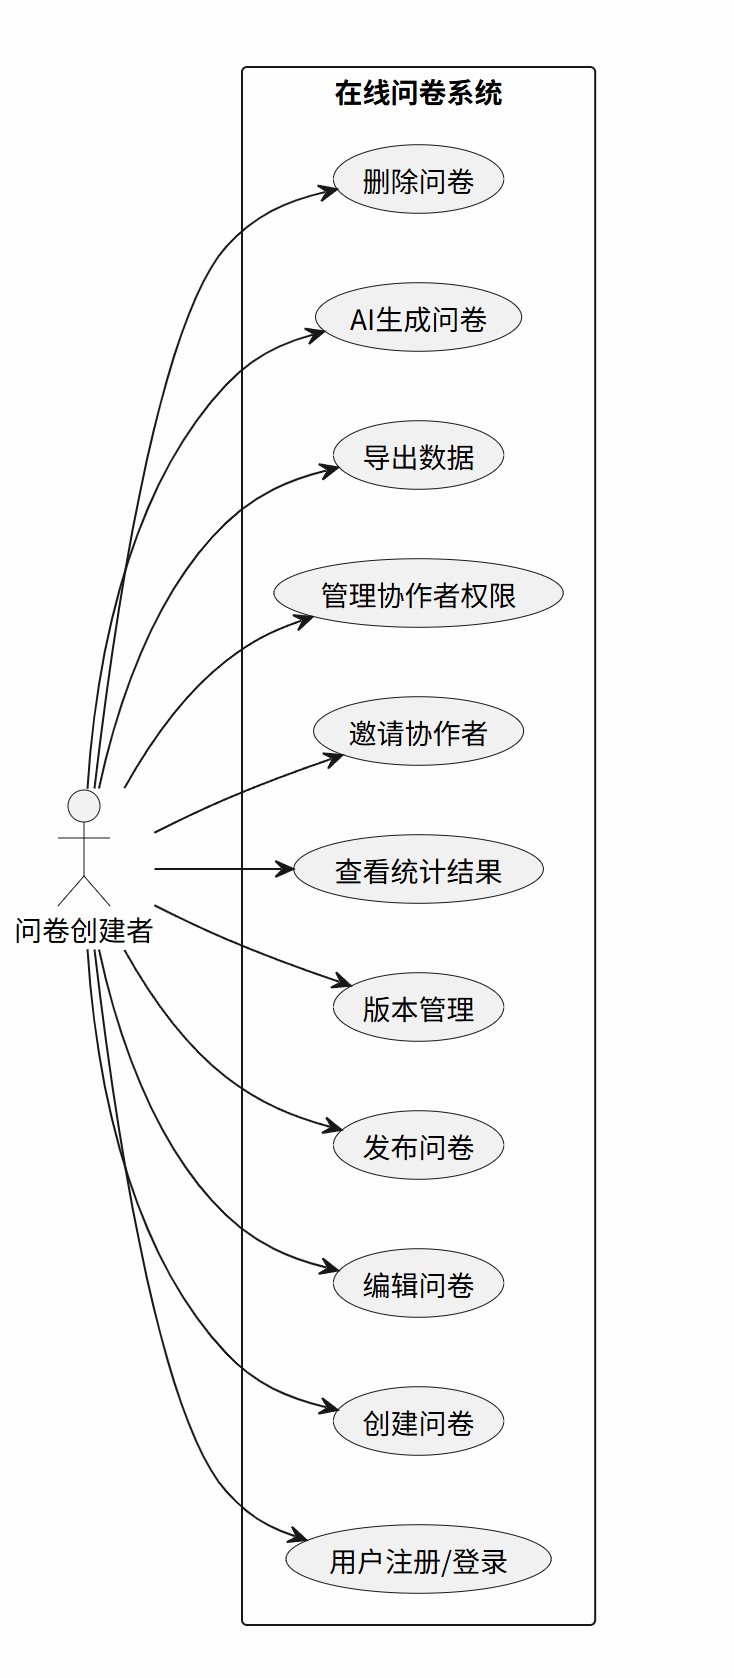
\includegraphics[width=0.55\textwidth]{figures/use-case-creator.png}
\caption{问卷创建者用例图}
\label{fig:use-case-creator}
\end{figure}

\subsubsection{问卷填写者需求分析}

问卷填写者通过公开链接访问问卷，其核心需求是流畅地完成答题并提交。
如图~\ref{fig:use-case-respondent} 所示，具体功能需求包括：

\begin{itemize}
  \item \textbf{访问问卷}：通过 \texttt{/s/\{shareToken\}} 链接访问已发布的问卷；
  \item \textbf{浏览题目}：查看问卷标题、描述及各题目内容；
  \item \textbf{填写答案}：根据题型要求选择或输入答案，系统提供前端必填校验；
  \item \textbf{提交问卷}：完成答题后提交，系统返回提交成功确认。
\end{itemize}

\begin{figure}[H]
\centering
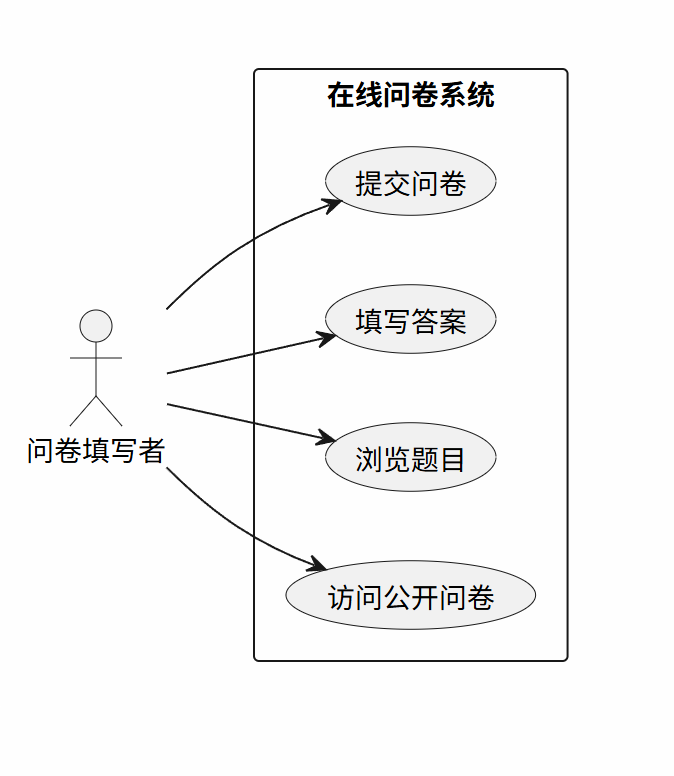
\includegraphics[width=0.75\textwidth]{figures/use-case-respondent.png}
\caption{问卷填写者用例图}
\label{fig:use-case-respondent}
\end{figure}

\subsubsection{协作者需求分析}

协作者受创建者邀请参与问卷协作，根据被授予的权限分为"可编辑"和
"可查看结果"两类。如图~\ref{fig:use-case-collaborator} 所示，
其功能需求包括：

\begin{itemize}
  \item \textbf{加入协作}：通过邀请码或邀请链接加入问卷协作，确认加入后获得相应权限；
  \item \textbf{编辑问卷}：在编辑器中查看和修改问卷内容（需具备编辑权限）；
  \item \textbf{实时协作}：参与多人实时协作编辑，系统通过题目级乐观锁定避免冲突，实时同步题目增删改、重排等变更；
  \item \textbf{查看结果}：查看问卷统计数据和可视化图表（需具备查看结果权限）。
\end{itemize}

\begin{figure}[H]
\centering
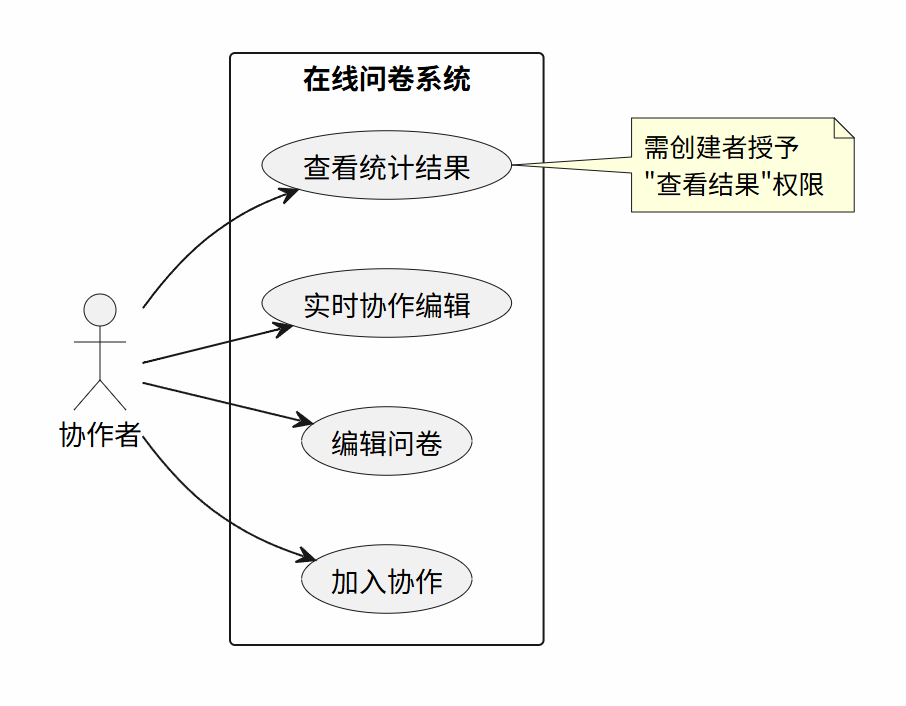
\includegraphics[width=0.55\textwidth]{figures/use-case-collaborator.png}
\caption{协作者用例图}
\label{fig:use-case-collaborator}
\end{figure}

\subsection{非功能需求分析}

除上述功能需求外，系统还需满足以下非功能需求，以保障系统的稳定性、
安全性和用户体验：

\begin{table}[H]
\centering
\caption{系统非功能需求}
\label{tab:non-functional-requirements}
\begin{tabular}{lp{10cm}}
\toprule
\textbf{需求类型} & \textbf{具体要求} \\
\midrule
性能 & 页面首屏加载时间 $<$ 3s，API 响应时间 $<$ 500ms，
编辑器首屏加载时间 $<$ 2.5s \\
可用性 & 系统可用性 $>$ 99\%，支持并发用户访问，
Pusher 实时协作延迟 $<$ 200ms \\
安全性 & 用户密码 bcrypt 加密存储（cost=12），
API JWT 鉴权，SQL 注入防护，HTTPS 传输 \\
可扩展性 & 模块化架构，题型注册中心模式支持新题型即插即用，
功能模块松耦合 \\
兼容性 & 支持主流桌面浏览器（Chrome、Firefox、Safari、Edge），
问卷填写页适配移动端 \\
\bottomrule
\end{tabular}
\end{table}

\subsection{本章小结}

本章对基于 Next.js 的在线问卷系统的需求进行了详细的分析。
首先明确了系统的业务背景与核心目标，指出现有平台在协作、
智能化和版本管理方面的不足。随后依据业务场景划分了三类目标用户：
问卷创建者、问卷填写者和协作者，并分别从各角色的视角出发，
详细分析了其功能需求，绘制了对应的用例图。
最后列出了系统的非功能需求，涵盖性能、可用性、安全性、
可扩展性和兼容性五个维度。

本章的需求分析为后续的系统架构设计、数据库设计和核心模块实现
奠定了基础，确保系统开发能够紧密围绕用户实际需求展开。

% ============================================
% 第4章 系统详细设计与实现
% ============================================
\section{系统详细设计与实现}

本章详细阐述系统各核心模块的设计思路与实现细节，包括问卷编辑器、发布与版本管理、填写与提交、结果统计、AI 辅助和实时协作等模块。

\subsection{问卷编辑器模块}

\subsubsection{编辑器整体架构}

问卷编辑器采用三栏布局设计：左侧为题型面板，中间为编辑画布，右侧为属性设置面板。\figref{fig:editor-layout} 展示了编辑器的界面布局。

\begin{figure}[H]
\centering
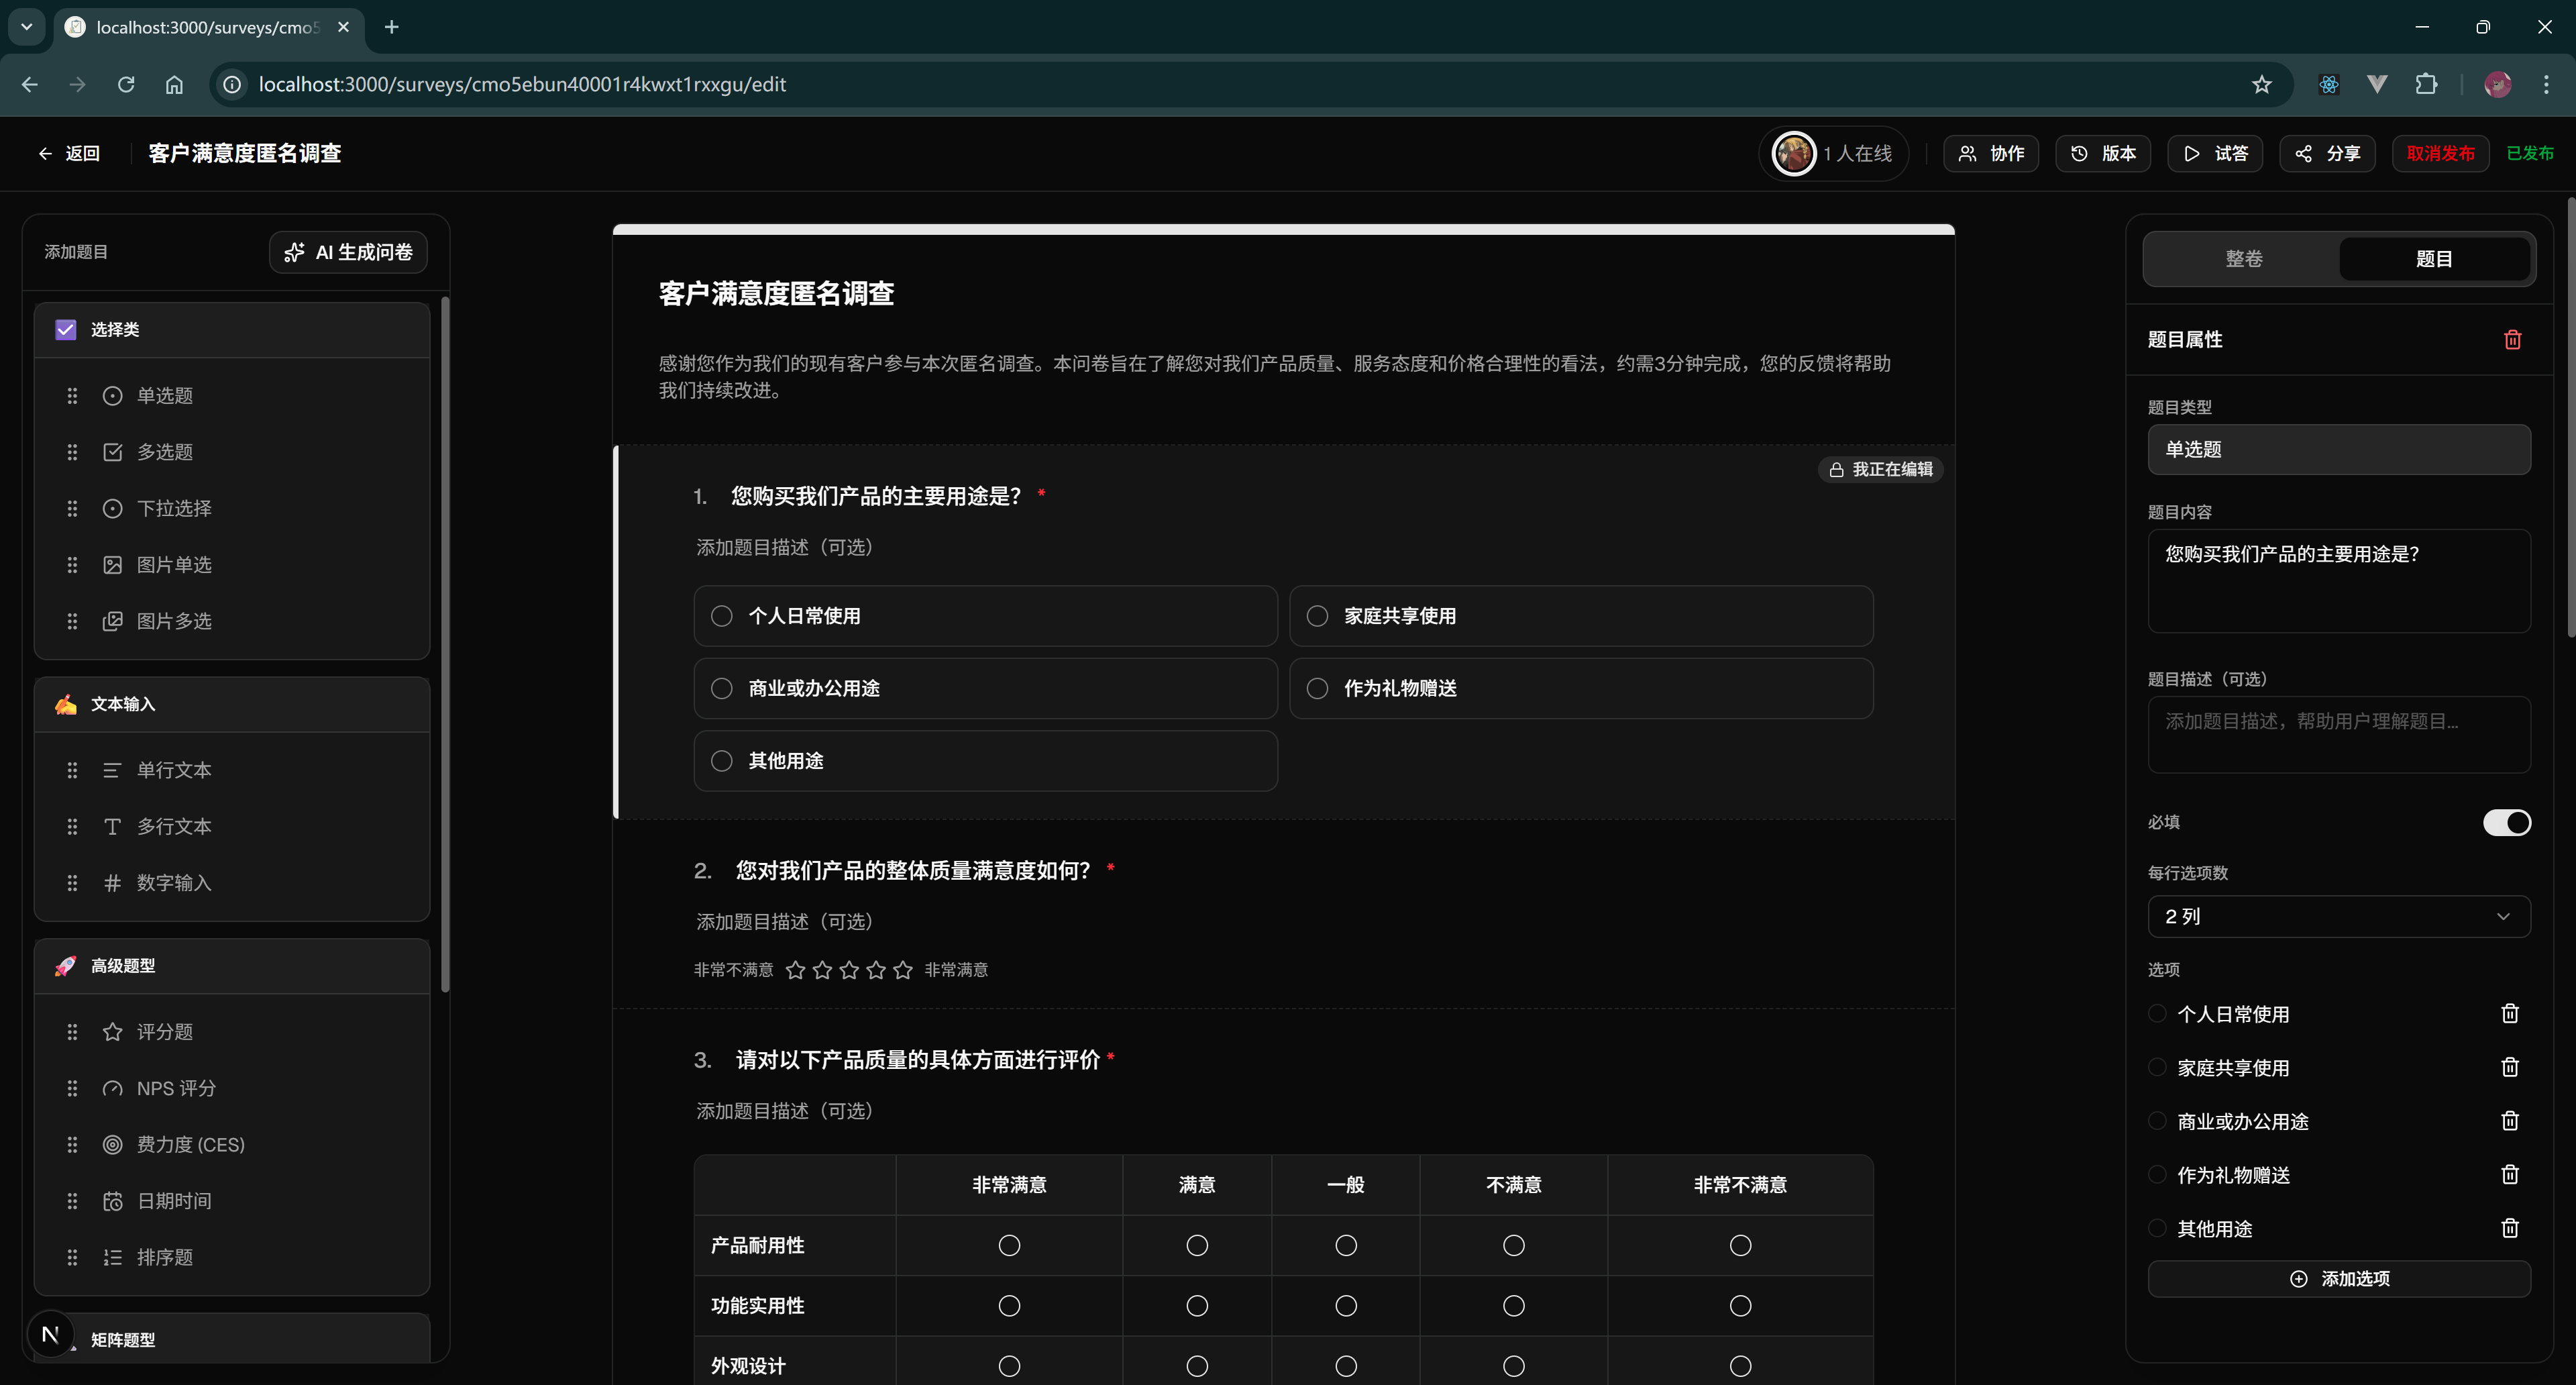
\includegraphics[width=0.95\textwidth]{figures/screenshot-editor.png}
\caption{问卷编辑器三栏布局}
\label{fig:editor-layout}
\end{figure}

\subsubsection{状态管理设计}

编辑器使用 Zustand 管理全局状态。Store 的核心结构如下：

\begin{lstlisting}[language=TypeScript, caption={编辑器 Zustand Store 结构}]
interface EditorState {
  // 问卷基本信息
  survey: Survey | null
  
  // 题目列表
  questions: Question[]
  
  // 当前选中题目
  selectedQuestionId: string | null
  
  // 编辑状态
  isLoading: boolean
  isSaving: boolean
  hasUnsavedChanges: boolean
  
  // Actions
  setSurvey: (survey: Survey) => void
  addQuestion: (type: QuestionType, index?: number) => void
  updateQuestion: (id: string, data: Partial<Question>) => void
  deleteQuestion: (id: string) => void
  reorderQuestions: (from: number, to: number) => void
  selectQuestion: (id: string | null) => void
}
\end{lstlisting}

Zustand 的不可变更新模式确保了 React 组件能够正确响应状态变化。以题目更新为例：

\begin{lstlisting}[language=TypeScript, caption={题目更新 Action 实现}]
updateQuestion: (id, data) => set((state) => ({
  questions: state.questions.map((q) =>
    q.id === id ? { ...q, ...data } : q
  ),
  hasUnsavedChanges: true,
})),
\end{lstlisting}

\subsubsection{题型系统}

系统支持 18 种题型，每种题型由四个核心部分组成：

\begin{enumerate}[label=(\arabic*)]
  \item \textbf{类型定义}：描述题型的数据结构
  \item \textbf{编辑器组件}：在编辑画布中渲染的配置界面
  \item \textbf{预览组件}：答题时的渲染界面
  \item \textbf{统计组件}：结果页中的数据展示
\end{enumerate}

题型通过注册中心统一管理：

\begin{lstlisting}[language=TypeScript, caption={题型注册中心}]
const questionRegistry: Record<QuestionType, QuestionDef> = {
  SINGLE_CHOICE: {
    type: 'SINGLE_CHOICE',
    label: '单选题',
    icon: CircleDot,
    editor: SingleChoiceEditor,
    preview: SingleChoicePreview,
    stats: SingleChoiceStats,
  },
  MULTIPLE_CHOICE: { /* ... */ },
  MATRIX_SINGLE: { /* ... */ },
  // ... 其他题型
}
\end{lstlisting}

\subsubsection{拖拽排序实现}

题目排序采用 HTML5 Drag and Drop API 实现。拖拽过程中需要处理以下事件：

\begin{lstlisting}[language=TypeScript, caption={拖拽排序核心逻辑}]
const handleDragStart = (e: DragEvent, index: number) => {
  e.dataTransfer?.setData('text/plain', String(index))
  setDraggedIndex(index)
}

const handleDrop = (e: DragEvent, targetIndex: number) => {
  const sourceIndex = Number(e.dataTransfer?.getData('text/plain'))
  if (sourceIndex === targetIndex) return
  
  reorderQuestions(sourceIndex, targetIndex)
  
  // 同步到服务器
  fetch(`/api/surveys/${surveyId}/questions/reorder`, {
    method: 'POST',
    body: JSON.stringify({ from: sourceIndex, to: targetIndex }),
  })
}
\end{lstlisting}

\subsubsection{行内编辑高度跳变问题}

在实现题目标题的行内编辑时，遇到了一个典型的 CSS 布局问题。当从预览态（\texttt{div}）切换到编辑态（\texttt{textarea}）时，父容器高度从 36px 跳变为 42.5px。

\textbf{根因分析}：\texttt{textarea} 默认是 \texttt{inline-block} 元素，浏览器会为文字的「降部」（descender）预留基线对齐空间，导致父容器被额外撑开。

\textbf{解决方案}：将 \texttt{textarea} 显式设置为 \texttt{display: block}，彻底脱离行内布局的基线对齐规则。

\begin{lstlisting}[language=CSS, caption={高度跳变问题修复}]
textarea.block {
  display: block;
  width: 100%;
}
\end{lstlisting}

\subsection{问卷发布与版本管理}

\subsubsection{发布流程设计}

问卷发布流程设计如下：

\begin{enumerate}[label=\textbf{\arabic*.}]
  \item 用户在编辑器中完成问卷内容编辑
  \item 点击「发布」按钮，触发版本创建
  \item 系统将当前问卷内容和题目快照保存为新的 \texttt{SurveyVersion} 记录
  \item 生成唯一的 \texttt{shareToken} 作为公开访问标识
  \item 问卷状态更新为已发布
\end{enumerate}

\subsubsection{版本快照机制}

每次发布时，系统将问卷的完整状态序列化为 JSON 存储：

\begin{lstlisting}[language=TypeScript, caption={版本快照创建}]
const version = await prisma.surveyVersion.create({
  data: {
    surveyId,
    version: nextVersionNumber,
    title: survey.title,
    questions: survey.questions.map(q => ({
      id: q.id,
      type: q.type,
      title: q.title,
      required: q.required,
      options: q.options,
      config: q.config,
    })),
  },
})

// 更新问卷的当前版本
await prisma.survey.update({
  where: { id: surveyId },
  data: { currentVersionId: version.id, published: true },
})
\end{lstlisting}

\subsubsection{版本回滚}

版本回滚将问卷内容恢复到指定版本的状态：

\begin{lstlisting}[language=TypeScript, caption={版本回滚实现}]
const rollbackVersion = async (surveyId: string, versionId: string) => {
  const version = await prisma.surveyVersion.findUnique({
    where: { id: versionId },
  })
  
  // 恢复问卷标题
  await prisma.survey.update({
    where: { id: surveyId },
    data: { title: version.title },
  })
  
  // 删除现有题目，重建版本中的题目
  await prisma.question.deleteMany({ where: { surveyId } })
  await prisma.question.createMany({
    data: version.questions.map((q, i) => ({
      surveyId,
      type: q.type,
      title: q.title,
      required: q.required,
      order: i,
      config: q.config,
    })),
  })
}
\end{lstlisting}

\subsubsection{已知问题与处理}

开发过程中发现，问卷列表页的「快速发布」按钮直接切换 \texttt{published} 状态，但未创建 \texttt{SurveyVersion} 记录。这导致用户提交答案时 \texttt{versionId} 为空，触发数据库外键约束错误。

\textbf{当前处理}：隐藏列表页的发布按钮，强制用户通过编辑器中的「版本管理」弹窗进行规范发布。

\textbf{根本修复方向}：统一发布入口，或在 \texttt{publish} API 中自动创建首个版本（如果尚无版本）。

\subsection{问卷填写与提交模块}

\subsubsection{公开问卷访问}

公开问卷通过 \texttt{shareToken} 访问，URL 格式为 \texttt{/s/\{token\}}。系统通过以下流程处理访问请求：

\begin{enumerate}[label=\textbf{\arabic*.}]
  \item 从 URL 中提取 \texttt{shareToken}
  \item 查询对应的问卷和当前版本
  \item 验证问卷是否已发布
  \item 返回问卷数据和题目列表
  \item 记录浏览量（24 小时内同一 IP 去重）
\end{enumerate}

\subsubsection{答案数据结构}

不同题型的答案存储格式不同：

\begin{table}[H]
\centering
\caption{各题型答案存储格式}
\label{tab:answer-formats}
\begin{tabular}{lll}
\toprule
\textbf{题型} & \textbf{存储格式} & \textbf{示例} \\
\midrule
单选题 & 字符串（选项 label） & \texttt{"非常同意"} \\
多选题 & 字符串数组 & \texttt{["选项A", "选项B"]} \\
文本题 & 字符串 & \texttt{"用户输入内容"} \\
评分题 & 数字 & \texttt{4} \\
矩阵单选 & 对象（rowId $\rightarrow$ colId） & \texttt{\{"q1": "col1"\}} \\
GENDER & 字符串（选项 ID） & \texttt{"male"} \\
\bottomrule
\end{tabular}
\end{table}

\subsubsection{提交 API 的 Schema 设计}

提交 API 使用 Zod 进行严格的类型校验。由于答案格式多样，Schema 需要支持多种类型：

\begin{lstlisting}[language=TypeScript, caption={提交 API Zod Schema}]
const submitSchema = z.object({
  answers: z.record(z.string(), z.union([
    z.string(),
    z.array(z.string()),
    z.number(),
    z.null(),
    z.record(z.string(), z.string()), // MATRIX_SINGLE
  ])),
})
\end{lstlisting}

\textbf{矩阵单选题的特殊处理}：矩阵单选题的答案是一个对象（\texttt{\{rowId: colId\}}），因此在 Zod Schema 中需要额外添加 \texttt{z.record(z.string(), z.string())} 类型支持。

\subsubsection{设备与地理位置采集}

系统在提交时自动采集以下信息：

\begin{itemize}
  \item \textbf{设备信息}：通过 User-Agent 解析设备类型、操作系统、浏览器
  \item \textbf{地理位置}：通过 IP 地址解析国家、省份、城市
  \item \textbf{来源渠道}：通过 \texttt{referrer} 或 URL 参数识别
\end{itemize}

地理位置通过 ip-api.com 免费 API 解析。在生产环境（HTTPS）下，由于浏览器安全策略限制，需要通过服务器代理转发请求。

\subsection{结果统计与可视化模块}

\subsubsection{统计页面架构}

结果统计页面采用侧边栏导航 + 内容区的布局，包含五个视图：

\begin{enumerate}[label=(\arabic*)]
  \item \textbf{数据概览}：KPI 卡片、回收趋势、设备/OS 分布、地域分布
  \item \textbf{数据详情}：回答表格、搜索筛选、分页、CSV 导出
  \item \textbf{统计图表}：逐题分析、多种图表类型切换
  \item \textbf{交叉分析}：两题交叉透视表
  \item \textbf{AI 总结}：智能数据分析报告（独立页面）
\end{enumerate}

\subsubsection{逐题统计实现}

逐题统计根据题型选择不同的展示方式：

\begin{lstlisting}[language=TypeScript, caption={逐题统计组件}]
const QuestionStats = ({ question, responses }: Props) => {
  switch (question.type) {
    case 'SINGLE_CHOICE':
    case 'MULTIPLE_CHOICE':
      return <ChoiceStats question={question} responses={responses} />
    case 'RATING':
    case 'NPS':
      return <RatingStats question={question} responses={responses} />
    case 'MATRIX_SINGLE':
      return <MatrixStats question={question} responses={responses} />
    case 'TEXT':
      return <TextStats question={question} responses={responses} />
    default:
      return <GenericStats question={question} responses={responses} />
  }
}
\end{lstlisting}

\subsubsection{GENDER 题型计数逻辑}

统计图表中 GENDER 题型的选项计数曾出现始终为 0 的问题。

\textbf{根因}：大多数选择题的答案存储的是选项 \textbf{label}，而 GENDER 题型特殊，存储的是选项 \textbf{ID}（\texttt{male}/\texttt{female}/\texttt{other}）。统计代码统一使用 \texttt{opt.label} 匹配，导致 GENDER 无法命中。

\textbf{修复}：在统计组件中增加类型判断：

\begin{lstlisting}[language=TypeScript, caption={GENDER 计数修复}]
const matchKey = type === 'GENDER' ? 'id' : 'label'
const count = counts[opt[matchKey]] || 0
\end{lstlisting}

\subsection{AI 辅助模块}

\subsubsection{AI 问卷生成}

AI 问卷生成采用「需求澄清 → 结构化生成」的两阶段流程：

\textbf{阶段一：需求澄清}

系统首先判断用户提供的信息是否足够生成问卷。如果信息不足，返回 1-3 个追问问题：

\begin{lstlisting}[language=TypeScript, caption={需求澄清流程}]
const clarifyResult = await generateObject({
  model: deepseek('deepseek-chat'),
  schema: clarifySchema,
  prompt: `判断以下需求是否足够生成问卷：${userInput}
  如果不足，请提出 1-3 个关键追问。`,
})

if (!clarifyResult.object.isSufficient) {
  return { questions: clarifyResult.object.followUpQuestions }
}
\end{lstlisting}

\textbf{阶段二：结构化生成}

信息充足后，调用 \texttt{generateObject} 生成结构化的问卷数据：

\begin{lstlisting}[language=TypeScript, caption={问卷生成实现}]
const result = await generateObject({
  model: deepseek('deepseek-chat'),
  schema: surveySchema, // Zod Schema 定义问卷结构
  prompt: `根据以下需求生成问卷：${userInput}
  要求：
  - 题目数量适中（5-15题）
  - 题型选择合理
  - 选项覆盖全面`,
})
\end{lstlisting}

\subsubsection{AI 数据总结}

AI 数据总结基于问卷回答数据生成分析报告：

\begin{lstlisting}[language=TypeScript, caption={AI 数据总结流程}]
// 1. 格式化数据为自然语言文本
const formattedData = formatSurveyData(survey, responses)

// 2. 调用 DeepSeek 流式生成
const result = streamText({
  model: deepseek('deepseek-chat'),
  system: '你是一位资深数据分析师...',
  prompt: formattedData,
})

// 3. 返回流式响应
return result.toDataStreamResponse()
\end{lstlisting}

\subsubsection{本地缓存策略}

为避免重复调用 AI API，系统实现了本地缓存：

\begin{lstlisting}[language=TypeScript, caption={AI 总结缓存实现}]
const useSummaryCache = (surveyId: string) => {
  const key = `ai-summary:${surveyId}`
  
  const get = () => {
    const raw = localStorage.getItem(key)
    if (!raw) return null
    const cached = JSON.parse(raw)
    // 当回答数变化时自动失效
    if (cached.totalResponses !== currentTotal) return null
    return cached.content
  }
  
  const set = (content: string, totalResponses: number) => {
    localStorage.setItem(key, JSON.stringify({
      content, totalResponses, timestamp: Date.now()
    }))
  }
  
  return { get, set }
}
\end{lstlisting}

\textbf{当前状态}：AI 总结页面功能完整，但鉴于数据量较小时生成质量不稳定，已暂时从侧边栏隐藏入口，保留页面代码供后续优化。

\subsection{实时协作模块}

\subsubsection{协作架构}

实时协作基于 Pusher 的 Presence Channel 实现。每个问卷对应一个独立的 Presence Channel，频道名格式为 \texttt{presence-survey-\{surveyId\}}。

\begin{figure}[H]
\centering
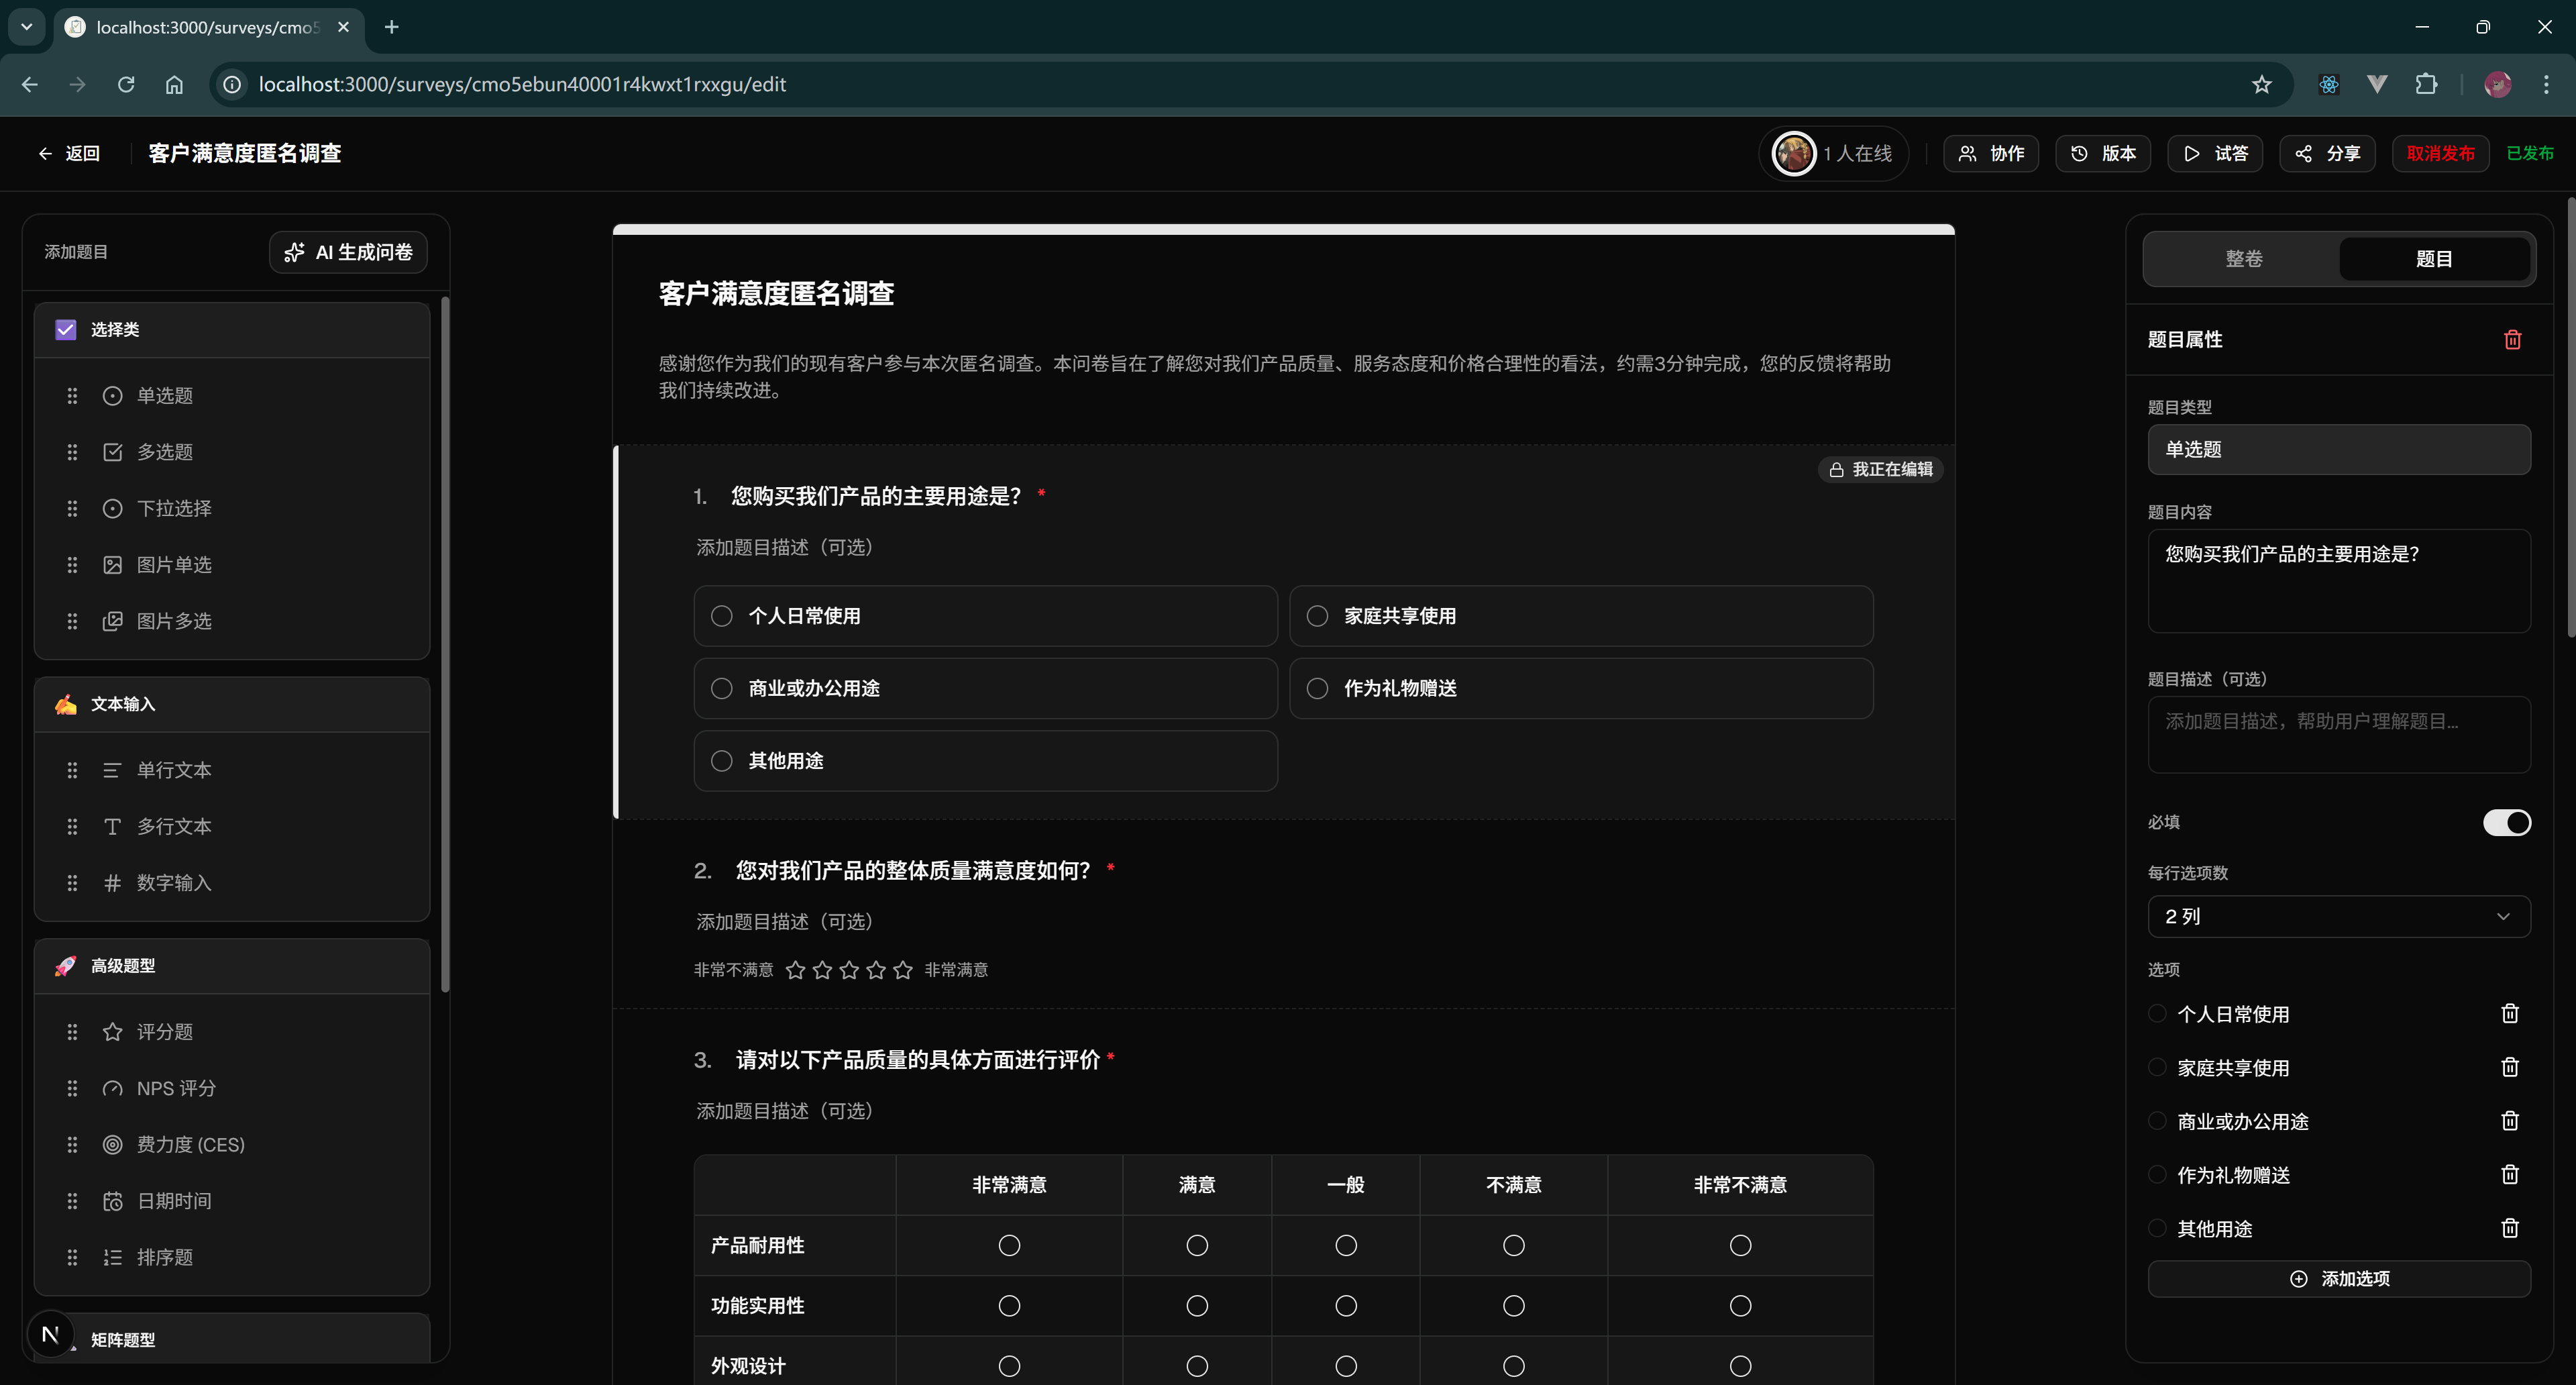
\includegraphics[width=0.95\textwidth]{figures/screenshot-editor.png}
\caption{实时协作编辑界面}
\label{fig:collaboration-arch}
\end{figure}

\subsubsection{题目乐观锁定}

为防止多人同时编辑同一题目，系统实现了题目级的乐观锁定：

\begin{lstlisting}[language=TypeScript, caption={题目锁定机制}]
// 选中题目时发送锁定请求
const lockQuestion = async (questionId: string) => {
  await fetch('/api/surveys/collaboration/lock', {
    method: 'POST',
    body: JSON.stringify({ surveyId, questionId }),
  })
  
  // 广播锁定事件
  channel.trigger('client-question-locked', {
    questionId,
    userId: currentUser.id,
    userName: currentUser.name,
  })
}

// 切换题目时释放锁定
const unlockQuestion = async (questionId: string) => {
  await fetch('/api/surveys/collaboration/unlock', {
    method: 'POST',
    body: JSON.stringify({ surveyId, questionId }),
  })
}
\end{lstlisting}

\subsubsection{实时同步事件}

系统通过以下事件实现状态同步：

\begin{table}[H]
\centering
\caption{Pusher 事件定义}
\label{tab:pusher-events}
\begin{tabular}{lll}
\toprule
\textbf{事件名} & \textbf{方向} & \textbf{说明} \\
\midrule
\texttt{question-locked} & client $\rightarrow$ client & 题目被锁定 \\
\texttt{question-unlocked} & client $\rightarrow$ client & 题目解锁 \\
\texttt{question-added} & client $\rightarrow$ client & 新增题目 \\
\texttt{question-updated} & client $\rightarrow$ client & 题目内容更新 \\
\texttt{question-deleted} & client $\rightarrow$ client & 删除题目 \\
\texttt{questions-reordered} & client $\rightarrow$ client & 题目重排 \\
\texttt{survey-updated} & client $\rightarrow$ client & 问卷信息更新 \\
\bottomrule
\end{tabular}
\end{table}

\subsubsection{异常处理}

系统处理了以下协作异常场景：

\begin{itemize}
  \item \textbf{成员意外离开}：通过 Presence Channel 的 \texttt{member-removed} 事件检测，自动释放该成员锁定的所有题目
  \item \textbf{网络断开重连}：Pusher 自动处理重连，恢复频道订阅
  \item \textbf{并发编辑冲突}：乐观锁定机制确保同一时刻只有一个用户编辑特定题目
\end{itemize}

\begin{lstlisting}[language=TypeScript, caption={成员离开自动解锁}]
channel.bind('pusher:member_removed', (member) => {
  // 释放该成员锁定的所有题目
  fetch('/api/surveys/collaboration/unlock-all', {
    method: 'POST',
    body: JSON.stringify({ surveyId, userId: member.id }),
  })
})
\end{lstlisting}

% ============================================
% 第5章 系统测试
% ============================================
\section{系统测试}

本章对系统进行全面的功能测试、性能测试和兼容性测试，验证系统是否满足设计需求。

\subsection{测试环境}

\begin{table}[H]
\centering
\caption{测试环境配置}
\label{tab:test-env}
\begin{tabular}{ll}
\toprule
\textbf{项目} & \textbf{配置} \\
\midrule
操作系统 & Windows 11 / macOS Sonoma \\
浏览器 & Chrome 120, Firefox 121, Safari 17, Edge 120 \\
Node.js & 20.x LTS \\
数据库 & PostgreSQL 15 (Neon 托管) \\
网络 & 100Mbps 宽带 / 5G 移动网络 \\
\bottomrule
\end{tabular}
\end{table}

\subsection{功能测试}

\subsubsection{用户认证测试}

\begin{table}[H]
\centering
\caption{用户认证功能测试用例}
\label{tab:auth-test}
\begin{tabular}{p{3cm}p{4cm}p{3cm}p{2cm}}
\toprule
\textbf{测试项} & \textbf{操作步骤} & \textbf{预期结果} & \textbf{结果} \\
\midrule
邮箱注册 & 填写邮箱、密码，点击注册 & 注册成功，跳转登录页 & 通过 \\
邮箱登录 & 输入正确邮箱密码 & 登录成功，跳转仪表盘 & 通过 \\
错误密码登录 & 输入错误密码 & 提示密码错误 & 通过 \\
Google OAuth & 点击 Google 登录按钮 & 跳转授权，登录成功 & 通过 \\
GitHub OAuth & 点击 GitHub 登录按钮 & 跳转授权，登录成功 & 通过 \\
未登录访问 & 直接访问 /surveys & 重定向到登录页 & 通过 \\
\bottomrule
\end{tabular}
\end{table}

\subsubsection{问卷编辑测试}

\begin{table}[H]
\centering
\caption{问卷编辑功能测试用例}
\label{tab:editor-test}
\begin{tabular}{p{3cm}p{4cm}p{3cm}p{2cm}}
\toprule
\textbf{测试项} & \textbf{操作步骤} & \textbf{预期结果} & \textbf{结果} \\
\midrule
创建问卷 & 点击新建，输入标题 & 问卷创建成功 & 通过 \\
添加题目 & 从左侧面板选择题型 & 题目添加到画布 & 通过 \\
编辑题目 & 点击题目，修改标题 & 标题实时更新 & 通过 \\
拖拽排序 & 拖拽题目到目标位置 & 顺序改变并保存 & 通过 \\
删除题目 & 点击删除按钮 & 题目移除 & 通过 \\
切换题型 & 更改题目类型 & 选项和配置更新 & 通过 \\
\bottomrule
\end{tabular}
\end{table}

\subsubsection{问卷发布与填写测试}

\begin{table}[H]
\centering
\caption{问卷发布与填写测试用例}
\label{tab:publish-test}
\begin{tabular}{p{3cm}p{4cm}p{3cm}p{2cm}}
\toprule
\textbf{测试项} & \textbf{操作步骤} & \textbf{预期结果} & \textbf{结果} \\
\midrule
发布问卷 & 编辑器中点击发布 & 生成分享链接 & 通过 \\
公开访问 & 使用 shareToken 访问 & 正常显示问卷 & 通过 \\
填写提交 & 选择答案，点击提交 & 提交成功，显示感谢页 & 通过 \\
必填验证 & 不填必填题直接提交 & 提示必填 & 通过 \\
版本管理 & 发布新版本，查看历史 & 版本列表正确 & 通过 \\
版本回滚 & 选择旧版本回滚 & 内容恢复到旧版本 & 通过 \\
\bottomrule
\end{tabular}
\end{table}

\subsubsection{结果统计测试}

\begin{table}[H]
\centering
\caption{结果统计功能测试用例}
\label{tab:results-test}
\begin{tabular}{p{3cm}p{4cm}p{3cm}p{2cm}}
\toprule
\textbf{测试项} & \textbf{操作步骤} & \textbf{预期结果} & \textbf{结果} \\
\midrule
数据概览 & 进入结果页，查看概览 & KPI 数据正确 & 通过 \\
统计图表 & 切换到图表标签 & 逐题图表正确渲染 & 通过 \\
数据筛选 & 设置筛选条件 & 表格数据更新 & 通过 \\
CSV 导出 & 点击导出按钮 & 下载 CSV 文件 & 通过 \\
交叉分析 & 选择两题交叉 & 透视表正确 & 通过 \\
\bottomrule
\end{tabular}
\end{table}

\subsubsection{实时协作测试}

\begin{table}[H]
\centering
\caption{实时协作功能测试用例}
\label{tab:collab-test}
\begin{tabular}{p{3cm}p{4cm}p{3cm}p{2cm}}
\toprule
\textbf{测试项} & \textbf{操作步骤} & \textbf{预期结果} & \textbf{结果} \\
\midrule
邀请加入 & 生成邀请码，另一用户加入 & 协作者列表更新 & 通过 \\
在线列表 & 多用户同时打开编辑器 & 显示所有在线成员 & 通过 \\
题目锁定 & 用户 A 选中题目 & 用户 B 看到锁定状态 & 通过 \\
实时同步 & 用户 A 修改题目 & 用户 B 实时看到更新 & 通过 \\
成员离开 & 用户 A 关闭页面 & 用户 B 看到成员离开 & 通过 \\
自动解锁 & 用户 A 意外断开 & 题目自动解锁 & 通过 \\
\bottomrule
\end{tabular}
\end{table}

\subsection{性能测试}

\subsubsection{页面加载性能}

使用 Chrome DevTools Lighthouse 进行性能测试：

\begin{table}[H]
\centering
\caption{页面加载性能测试}
\label{tab:perf-test}
\begin{tabular}{lccc}
\toprule
\textbf{页面} & \textbf{首屏时间} & \textbf{Lighthouse 评分} & \textbf{JS 体积} \\
\midrule
登录页 & 1.2s & 95 & 85KB \\
问卷列表 & 1.5s & 92 & 120KB \\
编辑器 & 2.1s & 88 & 280KB \\
公开问卷 & 1.8s & 90 & 150KB \\
结果统计 & 2.3s & 87 & 310KB \\
\bottomrule
\end{tabular}
\end{table}

\subsubsection{API 响应性能}

使用 Apache Bench 进行 API 压力测试：

\begin{table}[H]
\centering
\caption{API 响应性能测试}
\label{tab:api-perf}
\begin{tabular}{lccc}
\toprule
\textbf{接口} & \textbf{平均响应} & \textbf{P95} & \textbf{并发 100} \\
\midrule
GET /api/surveys & 45ms & 120ms & 通过 \\
GET /api/surveys/{id} & 38ms & 95ms & 通过 \\
POST /api/s/{token}/submit & 85ms & 210ms & 通过 \\
GET /api/surveys/{id}/responses & 120ms & 350ms & 通过 \\
\bottomrule
\end{tabular}
\end{table}

\subsection{兼容性测试}

\begin{table}[H]
\centering
\caption{浏览器兼容性测试}
\label{tab:compat-test}
\begin{tabular}{lccccc}
\toprule
\textbf{功能} & \textbf{Chrome} & \textbf{Firefox} & \textbf{Safari} & \textbf{Edge} & \textbf{移动端} \\
\midrule
用户认证 & $\checkmark$ & $\checkmark$ & $\checkmark$ & $\checkmark$ & $\checkmark$ \\
问卷编辑 & $\checkmark$ & $\checkmark$ & $\checkmark$ & $\checkmark$ & $\triangle$ \\
拖拽排序 & $\checkmark$ & $\checkmark$ & $\checkmark$ & $\checkmark$ & $\times$ \\
问卷填写 & $\checkmark$ & $\checkmark$ & $\checkmark$ & $\checkmark$ & $\checkmark$ \\
结果统计 & $\checkmark$ & $\checkmark$ & $\checkmark$ & $\checkmark$ & $\checkmark$ \\
实时协作 & $\checkmark$ & $\checkmark$ & $\checkmark$ & $\checkmark$ & $\triangle$ \\
\bottomrule
\end{tabular}
\end{table}

注：$\checkmark$ 完全支持，$\triangle$ 部分支持，$\times$ 不支持。

\subsection{测试结果分析}

综合测试结果，系统功能完整，主要模块均通过测试。性能方面，页面加载时间和 API 响应时间均在可接受范围内。兼容性方面，系统支持主流桌面浏览器，移动端在问卷填写和结果查看方面表现良好，但编辑器因屏幕尺寸限制，移动端体验有待优化。

\textbf{发现的问题}：

\begin{enumerate}[label=(\arabic*)]
  \item 编辑器页面 JS 体积较大（280KB），可进一步优化代码分割
  \item 结果统计页面在数据量较大时（>10000 条回答）加载较慢，需要增加分页或聚合优化
  \item 移动端拖拽排序不支持，需要为移动端设计替代交互
\end{enumerate}

% ============================================
% 第6章 总结与展望
% ============================================
\section{总结与展望}

\subsection{工作总结}

本文设计并实现了一个基于 Next.js 的在线问卷系统，完成了以下主要工作：

\textbf{(1) 完整的问卷生命周期管理}

系统涵盖了问卷从创建、编辑、发布、收集到统计分析的完整生命周期。用户可以通过可视化编辑器灵活设计问卷，支持 18 种题型，满足不同场景的数据收集需求。

\textbf{(2) 版本管理机制}

设计了问卷版本管理系统，每次发布自动创建内容快照，支持版本历史查看和回滚操作。这一机制保障了问卷内容变更的可追溯性，避免了误操作导致的数据丢失。

\textbf{(3) AI 辅助功能}

集成 DeepSeek 大语言模型，实现了问卷智能生成和数据分析总结功能。通过需求澄清对话引导用户明确需求，利用结构化生成确保输出质量，并采用流式输出提升用户体验。

\textbf{(4) 实时协作编辑}

基于 Pusher 实现了多人实时协作编辑功能，支持题目级乐观锁定、在线成员列表、实时状态同步等特性。这一功能填补了现有问卷平台在协作方面的空白。

\textbf{(5) 数据可视化}

利用 ECharts 实现了多维度的数据统计和可视化展示，包括回收趋势、设备分布、地域分布、逐题统计和交叉分析等，帮助用户从数据中获取洞察。

\subsection{创新点}

本文的主要创新点包括：

\begin{enumerate}[label=(\arabic*)]
  \item \textbf{AI 深度集成}：将大语言模型与问卷系统深度结合，不仅支持问卷生成，还能基于实际回答数据进行智能分析总结，形成了「设计-收集-分析」的 AI 辅助闭环。
  
  \item \textbf{实时协作机制}：设计了基于 Presence Channel 的多人协作方案，通过题目级乐观锁定实现细粒度的并发控制，在保证协作体验的同时避免编辑冲突。
  
  \item \textbf{版本管理设计}：将版本快照与发布流程紧密结合，每次发布自动生成不可变快照，支持任意历史版本的查看和回滚，为问卷内容管理提供了可靠保障。
\end{enumerate}

\subsection{存在的不足}

尽管系统功能较为完善，但仍存在以下不足：

\begin{enumerate}[label=(\arabic*)]
  \item \textbf{AI 生成质量不稳定}：当问卷数据量较小时，AI 生成的总结内容较为空洞，需要进一步优化 prompt 设计和数据预处理策略。
  
  \item \textbf{移动端编辑器体验欠佳}：由于编辑器采用桌面端优化的三栏布局，在移动设备上操作不便，需要针对移动端重新设计交互。
  
  \item \textbf{大数据量性能瓶颈}：当单份问卷的回答数量超过一万条时，统计页面的加载和计算速度明显下降，需要引入数据预聚合或分页加载机制。
  
  \item \textbf{协作冲突处理简单}：当前的乐观锁定机制虽然避免了同时编辑同一题目的问题，但对于更复杂的冲突场景（如同时修改问卷设置）缺乏细粒度的处理策略。
\end{enumerate}

\subsection{未来展望}

针对上述不足，未来可以从以下方向进行改进：

\textbf{(1) AI 功能增强}

\begin{itemize}
  \item 引入 RAG（检索增强生成）技术，基于历史问卷数据提升生成质量
  \item 支持用户自定义分析维度，让 AI 总结更加精准
  \item 探索多模态输入，支持基于图片、文档生成问卷
\end{itemize}

\textbf{(2) 移动端优化}

\begin{itemize}
  \item 为移动端设计简化的编辑器界面
  \item 支持触摸手势操作（滑动、长按等）
  \item 开发配套的小程序或 App，提升移动端体验
\end{itemize}

\textbf{(3) 性能优化}

\begin{itemize}
  \item 引入 Redis 缓存热点数据，减少数据库查询压力
  \item 对统计数据进行预聚合，提升大数据量下的查询性能
  \item 优化前端代码分割策略，减少首屏加载时间
\end{itemize}

\textbf{(4) 协作功能完善}

\begin{itemize}
  \item 引入 OT 或 CRDT 算法，支持更细粒度的协同编辑
  \item 增加评论和批注功能，方便协作者之间沟通
  \item 支持协作历史回溯，查看谁在何时做了哪些修改
\end{itemize}

\textbf{(5) 功能扩展}

\begin{itemize}
  \item 支持问卷逻辑跳转（根据答案显示不同题目）
  \item 增加问卷模板市场，提供行业最佳实践
  \item 支持数据导出到 BI 工具（如 Power BI、Tableau）
  \item 增加问卷定时发布和自动关闭功能
\end{itemize}


% ---------- 参考文献 ----------
% ============================================
% 参考文献
% ============================================
\newpage
\section*{参考文献}
\addcontentsline{toc}{section}{参考文献}

\begin{enumerate}[label={[\arabic*]}, leftmargin=2em]

\item Vercel. Next.js Documentation[EB/OL]. https://nextjs.org/docs, 2024.

\item Meta Platforms, Inc. React Documentation[EB/OL]. https://react.dev, 2024.

\item Prisma Data, Inc. Prisma Documentation[EB/OL]. https://www.prisma.io/docs, 2024.

\item Pusher Ltd. Pusher Channels Documentation[EB/OL]. https://pusher.com/docs/channels, 2024.

\item Vercel. AI SDK Documentation[EB/OL]. https://sdk.vercel.ai/docs, 2024.

\item DeepSeek-AI. DeepSeek API Documentation[EB/OL]. https://platform.deepseek.com, 2024.

\item 百度 ECharts 团队. ECharts 文档[EB/OL]. https://echarts.apache.org, 2024.

\item Auth.js. Authentication for the Web[EB/OL]. https://authjs.dev, 2024.

\item Ihrig C J. Pro Node.js for Developers[M]. Berkeley: Apress, 2013.

\item Stoyan S. React: Up \& Running: Building Web Applications[M]. Sebastopol: O'Reilly Media, 2016.

\item 刘伟, 张华. 基于 Web 的在线问卷调查系统设计与实现[J]. 计算机应用与软件, 2019, 36(5): 78-83.

\item 李明, 王芳. 在线问卷系统的设计与实现[J]. 软件导刊, 2020, 19(8): 56-60.

\item Ellis C A, Gibbs S J. Concurrency Control in Groupware Systems[C]//ACM SIGMOD Record. ACM, 1989, 18(2): 399-407.

\item Shapiro M, Preguiça N, Baquero C, et al. Conflict-free Replicated Data Types[C]//Symposium on Self-Stabilizing Systems. Springer, 2011: 386-400.

\item 陈刚, 刘洋. 基于 React 的前端开发框架研究[J]. 计算机技术与发展, 2021, 31(3): 145-150.

\item 赵军, 孙伟. 基于 Node.js 的全栈 Web 应用开发技术研究[J]. 计算机工程与设计, 2020, 41(12): 3456-3461.

\item 周明, 吴强. 实时协作编辑系统关键技术研究综述[J]. 计算机学报, 2022, 45(6): 1234-1256.

\item 郑华, 黄磊. 大语言模型在智能问答系统中的应用研究[J]. 中文信息学报, 2023, 37(5): 1-15.

\item 林峰, 张杰. 基于 PostgreSQL 的数据库应用系统设计与优化[J]. 计算机系统应用, 2021, 30(9): 67-73.

\item 马云, 刘强. 数据可视化技术在商业智能中的应用[J]. 数据分析与知识发现, 2022, 6(4): 89-98.

\end{enumerate}


% ---------- 致谢 ----------
% ============================================
% 致谢
% ============================================
\newpage
\section*{致\quad 谢}
\addcontentsline{toc}{section}{致谢}

时光荏苒，四年的大学生活即将画上句号。在论文完成之际，我要向所有给予我帮助和支持的人表示衷心的感谢。

首先，我要感谢我的指导老师。从选题到开题，从系统设计到论文撰写，老师都给予了悉心的指导和耐心的帮助。老师严谨的治学态度和深厚的学术造诣让我受益匪浅。

感谢学院的各位老师，是你们传授给我扎实的专业知识和学习方法，为本次毕业设计的顺利完成奠定了基础。

感谢我的同学们，在四年的学习和生活中，我们互相帮助、共同进步。特别感谢在毕业设计期间与我讨论技术问题、分享开发经验的伙伴们。

感谢我的家人，是你们无私的支持和鼓励，让我能够专心完成学业。你们的理解和包容是我前进的动力。

最后，感谢所有参与系统测试和提供反馈意见的用户，你们的建议帮助我发现并改进了系统中的诸多问题。

由于时间和能力有限，本系统还存在许多不足之处，恳请各位老师批评指正。


% ---------- 附录 ----------
\appendix
% ============================================
% 附录
% ============================================
\section{附录 A：核心数据模型定义}

\subsection{用户认证模型}

\begin{minted}[linenos]{typescript}
model User {
  id            String    @id @default(cuid())
  name          String?
  email         String    @unique
  emailVerified DateTime?
  image         String?
  password      String?
  createdAt     DateTime  @default(now())
  updatedAt     DateTime  @updatedAt

  accounts       Account[]
  sessions       Session[]
  authenticators Authenticator[]
  surveys        Survey[]
  collaborations SurveyCollaborator[]
  surveyLogs     SurveyLog[]
}

model Account {
  id                String  @id @default(cuid())
  userId            String
  type              String
  provider          String
  providerAccountId String
  refresh_token     String? @db.Text
  access_token      String? @db.Text
  expires_at        Int?
  token_type        String?
  scope             String?
  id_token          String? @db.Text
  session_state     String?

  user User @relation(fields: [userId], references: [id], onDelete: Cascade)
  @@unique([provider, providerAccountId])
}
\end{minted}
\captionof{listing}{User 与 Account 模型}

\begin{minted}[linenos]{typescript}
model Session {
  id           String   @id @default(cuid())
  sessionToken String   @unique
  userId       String
  expires      DateTime
  user User @relation(fields: [userId], references: [id], onDelete: Cascade)
}

model Authenticator {
  credentialID         String  @unique
  userId               String
  providerAccountId    String
  credentialPublicKey  String
  counter              Int
  credentialDeviceType String
  credentialBackedUp   Boolean
  transports           String?
  user User @relation(fields: [userId], references: [id], onDelete: Cascade)
  @@unique([userId, credentialID])
}
\end{minted}
\captionof{listing}{Session 与 Authenticator 模型}

\subsection{问卷核心模型}

\begin{minted}[linenos]{typescript}
model Survey {
  id               String   @id @default(cuid())
  title            String
  description      String?
  published        Boolean  @default(false)
  shareToken       String   @unique @default(cuid())
  settings         Json?
  userId           String
  maxCollaborators Int      @default(10)
  currentVersionId String?
  createdAt        DateTime @default(now())
  updatedAt        DateTime @updatedAt

  user          User                 @relation(fields: [userId], references: [id], onDelete: Cascade)
  questions     Question[]
  responses     Response[]
  views         SurveyView[]
  collaborators SurveyCollaborator[]
  invites       SurveyInvite[]
  logs          SurveyLog[]
  versions      SurveyVersion[]
  @@index([currentVersionId])
}

model Question {
  id          String       @id @default(cuid())
  surveyId    String
  type        QuestionType
  title       String
  description String?
  required    Boolean      @default(false)
  order       Int
  config      Json?
  lockedBy    String?
  lockedAt    DateTime?
  survey  Survey   @relation(fields: [surveyId], references: [id], onDelete: Cascade)
  answers Answer[]
  @@index([lockedBy])
}
\end{minted}
\captionof{listing}{问卷与题目模型}

\begin{minted}[linenos]{typescript}
model SurveyVersion {
  id          String   @id @default(cuid())
  surveyId    String
  version     Int
  title       String
  description String?
  questions   Json
  publishedAt DateTime @default(now())
  createdAt   DateTime @default(now())
  survey    Survey     @relation(fields: [surveyId], references: [id], onDelete: Cascade)
  responses Response[]
  @@unique([surveyId, version])
  @@index([surveyId])
  @@index([publishedAt])
}

model Response {
  id          String   @id @default(cuid())
  surveyId    String
  versionId   String
  respondent  String?
  startedAt   DateTime?
  completedAt DateTime?
  createdAt   DateTime @default(now())
  survey  Survey        @relation(fields: [surveyId], references: [id], onDelete: Cascade)
  version SurveyVersion @relation(fields: [versionId], references: [id], onDelete: Cascade)
  answers Answer[]
  @@index([versionId])
  @@index([createdAt])
}

model Answer {
  id         String @id @default(cuid())
  responseId String
  questionId String
  value      Json
  response Response @relation(fields: [responseId], references: [id], onDelete: Cascade)
  question Question @relation(fields: [questionId], references: [id], onDelete: Cascade)
}
\end{minted}
\captionof{listing}{版本与回答模型}

\clearpage
\subsection{协作与日志模型}

\begin{minted}[linenos]{typescript}
model SurveyCollaborator {
  id             String @id @default(cuid())
  surveyId       String
  userId         String
  canEdit        Boolean @default(false)
  canViewResults Boolean @default(false)
  invitedBy      String
  createdAt      DateTime @default(now())
  survey Survey @relation(fields: [surveyId], references: [id], onDelete: Cascade)
  user   User   @relation(fields: [userId], references: [id], onDelete: Cascade)
  @@unique([surveyId, userId])
  @@index([surveyId])
  @@index([userId])
}

model SurveyInvite {
  id          String    @id @default(cuid())
  surveyId    String
  code        String    @unique
  maxUses     Int?
  usedCount   Int       @default(0)
  expiresAt   DateTime?
  permissions Json?
  createdBy   String
  createdAt   DateTime  @default(now())
  survey Survey @relation(fields: [surveyId], references: [id], onDelete: Cascade)
  @@index([surveyId])
  @@index([code])
}
\end{minted}
\captionof{listing}{协作者与邀请码模型}

\begin{minted}[linenos]{typescript}
model SurveyLog {
  id        String   @id @default(cuid())
  surveyId  String
  userId    String
  action    String
  details   Json?
  createdAt DateTime @default(now())
  survey Survey @relation(fields: [surveyId], references: [id], onDelete: Cascade)
  user   User   @relation(fields: [userId], references: [id], onDelete: Cascade)
  @@index([surveyId])
  @@index([createdAt])
}

model SurveyView {
  id         String   @id @default(cuid())
  surveyId   String
  viewedAt   DateTime @default(now())
  ip         String?
  deviceType String?
  os         String?
  browser    String?
  country    String?
  province   String?
  city       String?
  survey Survey @relation(fields: [surveyId], references: [id], onDelete: Cascade)
  @@index([surveyId])
  @@index([viewedAt])
}
\end{minted}
\captionof{listing}{操作日志与浏览记录模型}

\section{附录 B：系统界面截图}

\begin{figure}[H]
\centering
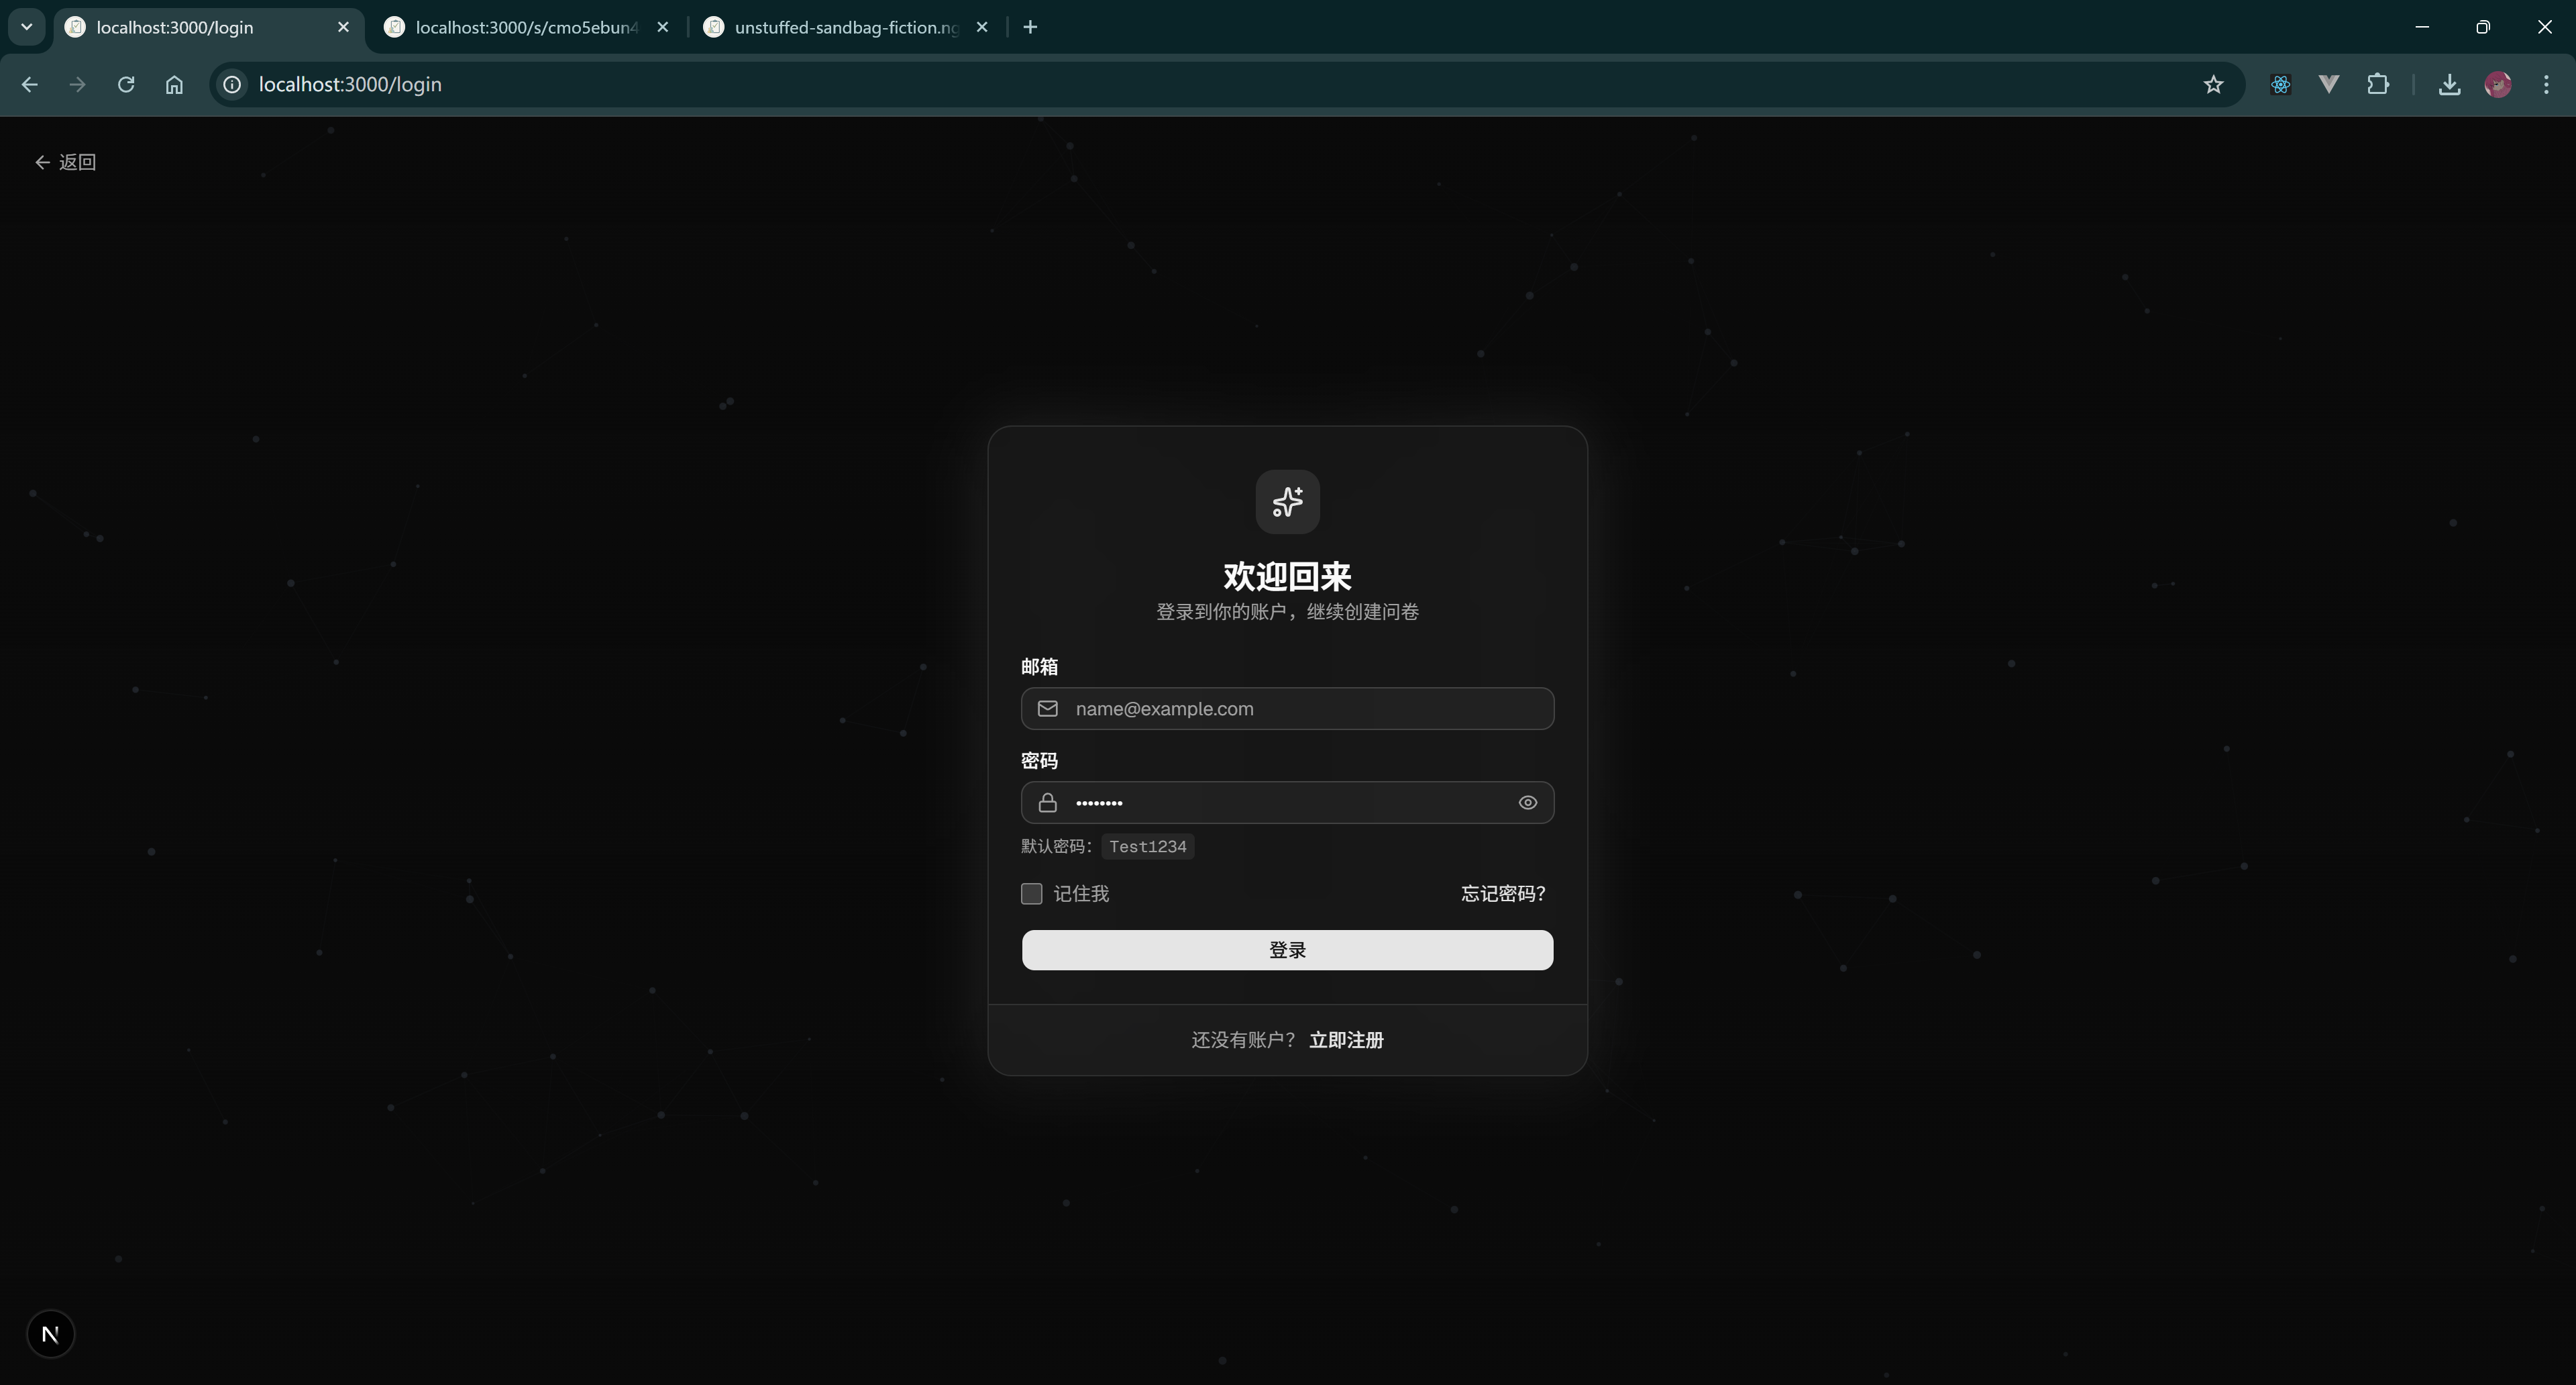
\includegraphics[width=0.95\textwidth]{figures/screenshot-login.png}
\caption{登录页面}
\end{figure}

\begin{figure}[H]
\centering
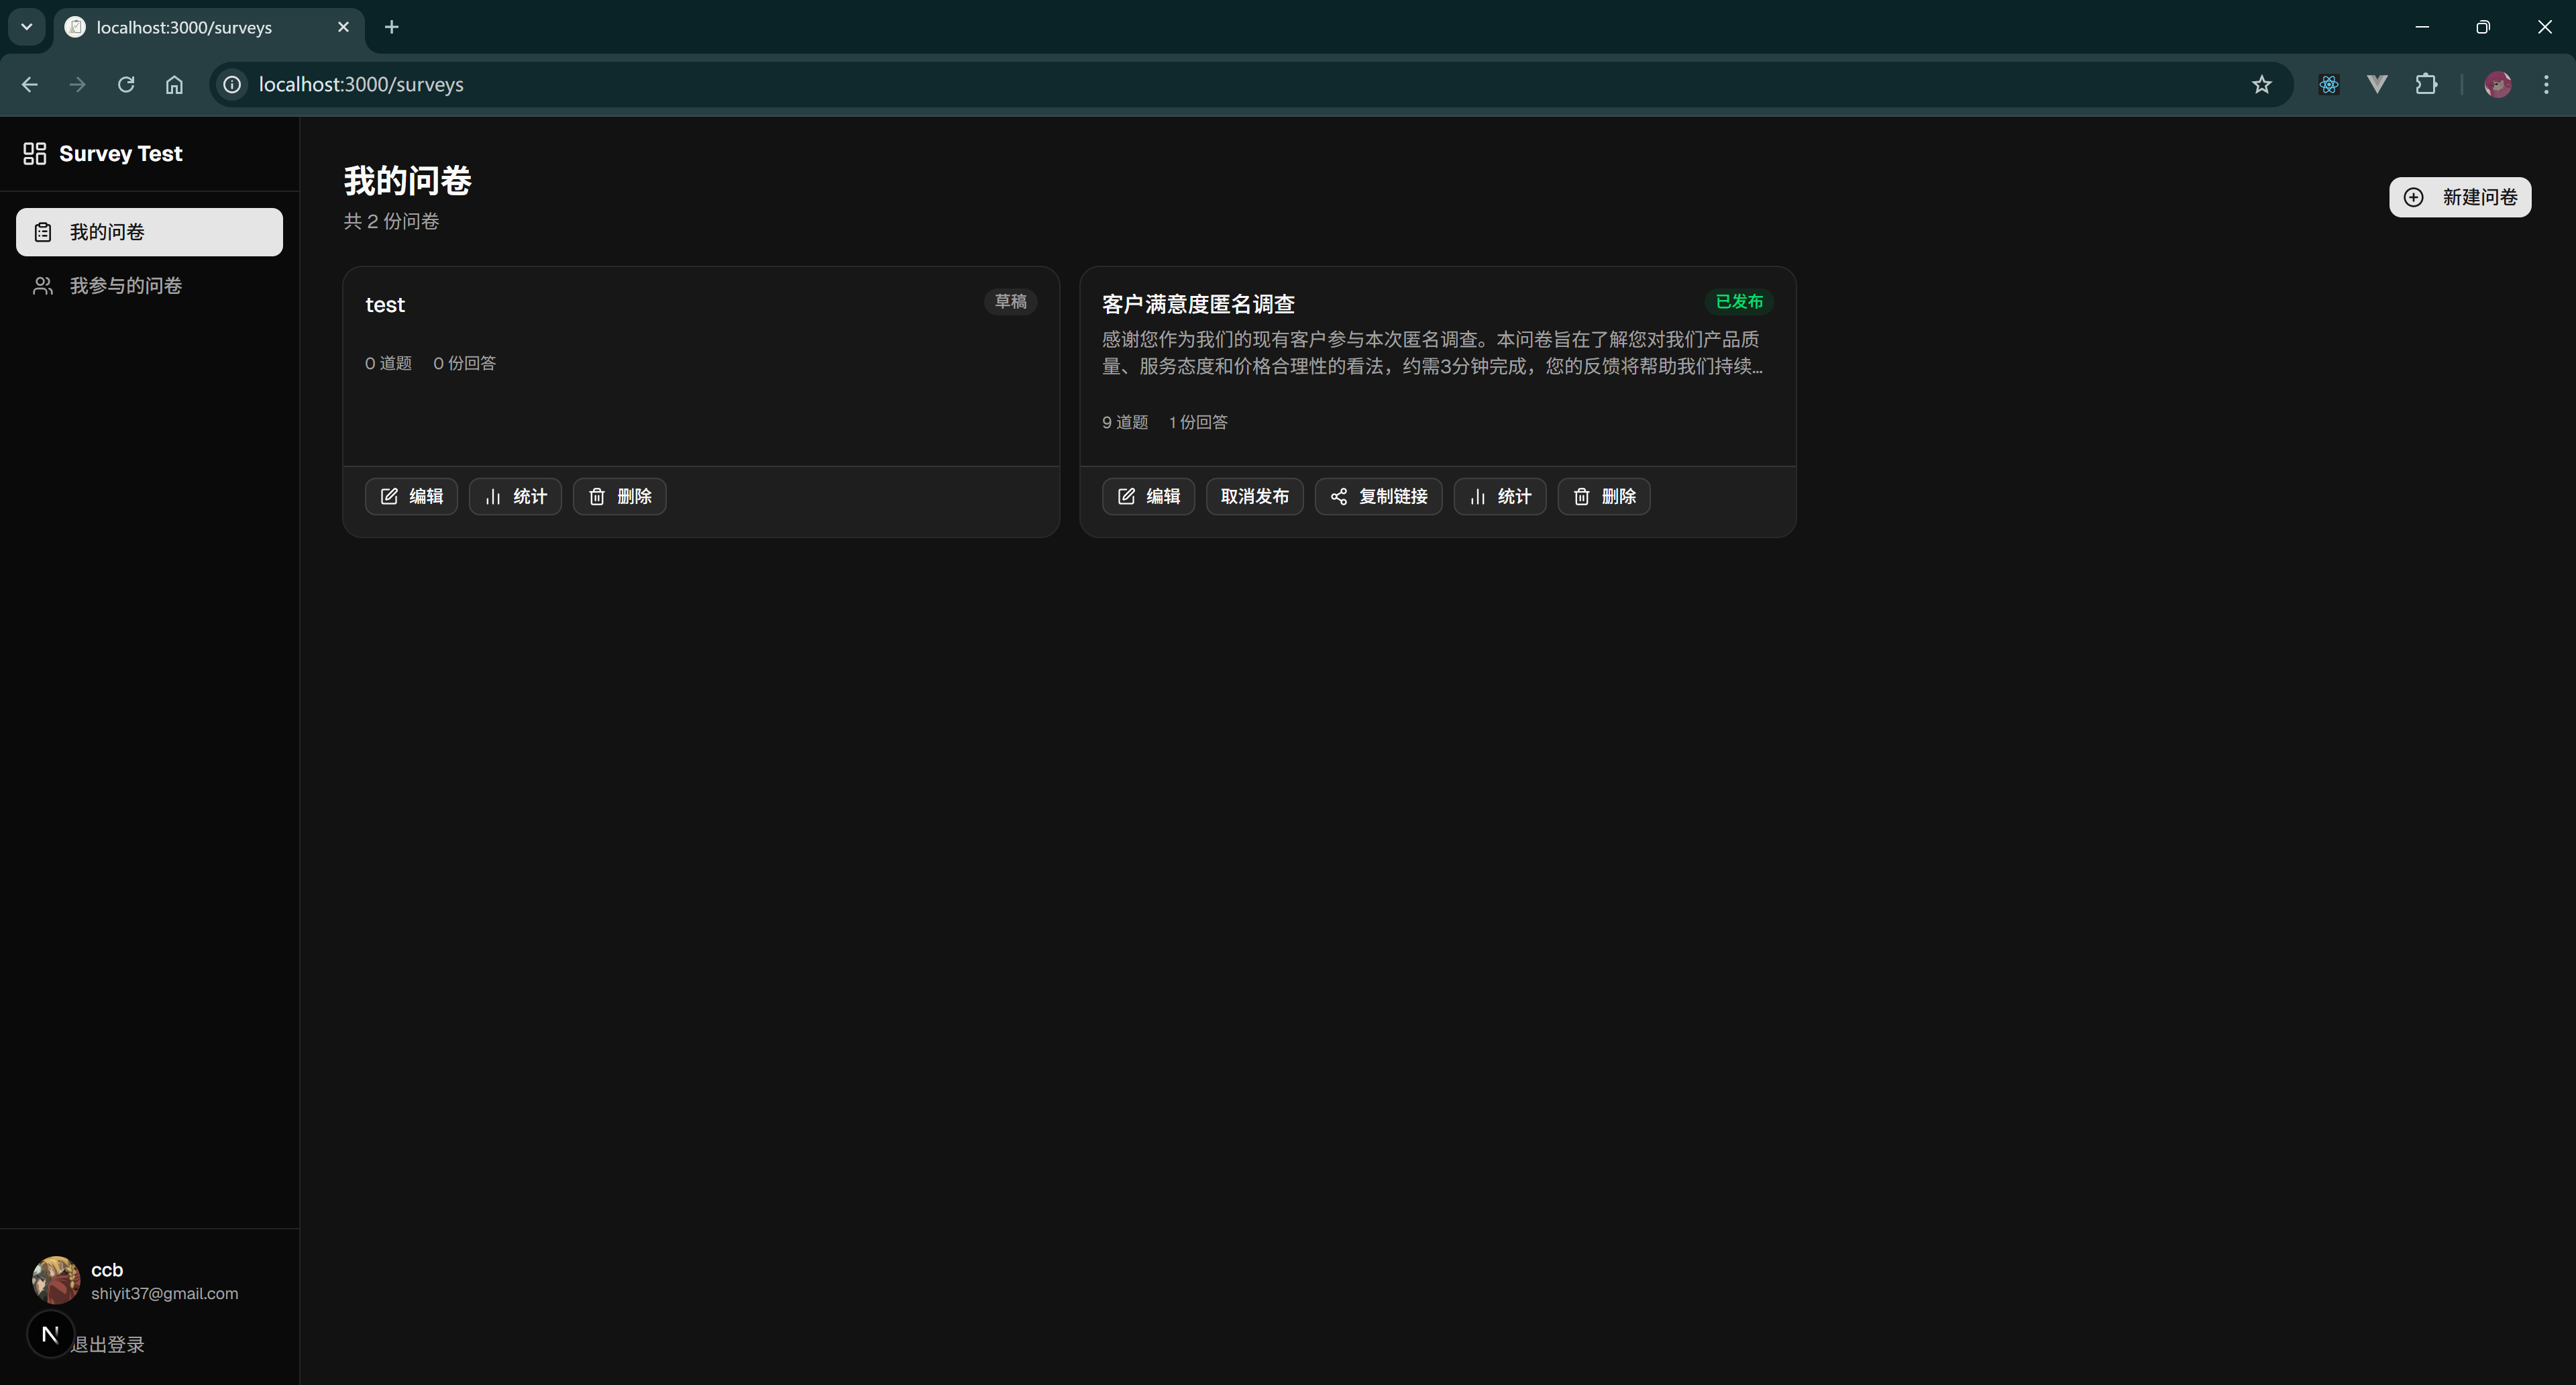
\includegraphics[width=0.95\textwidth]{figures/screenshot-survey-list.png}
\caption{问卷列表页面}
\end{figure}

\begin{figure}[H]
\centering
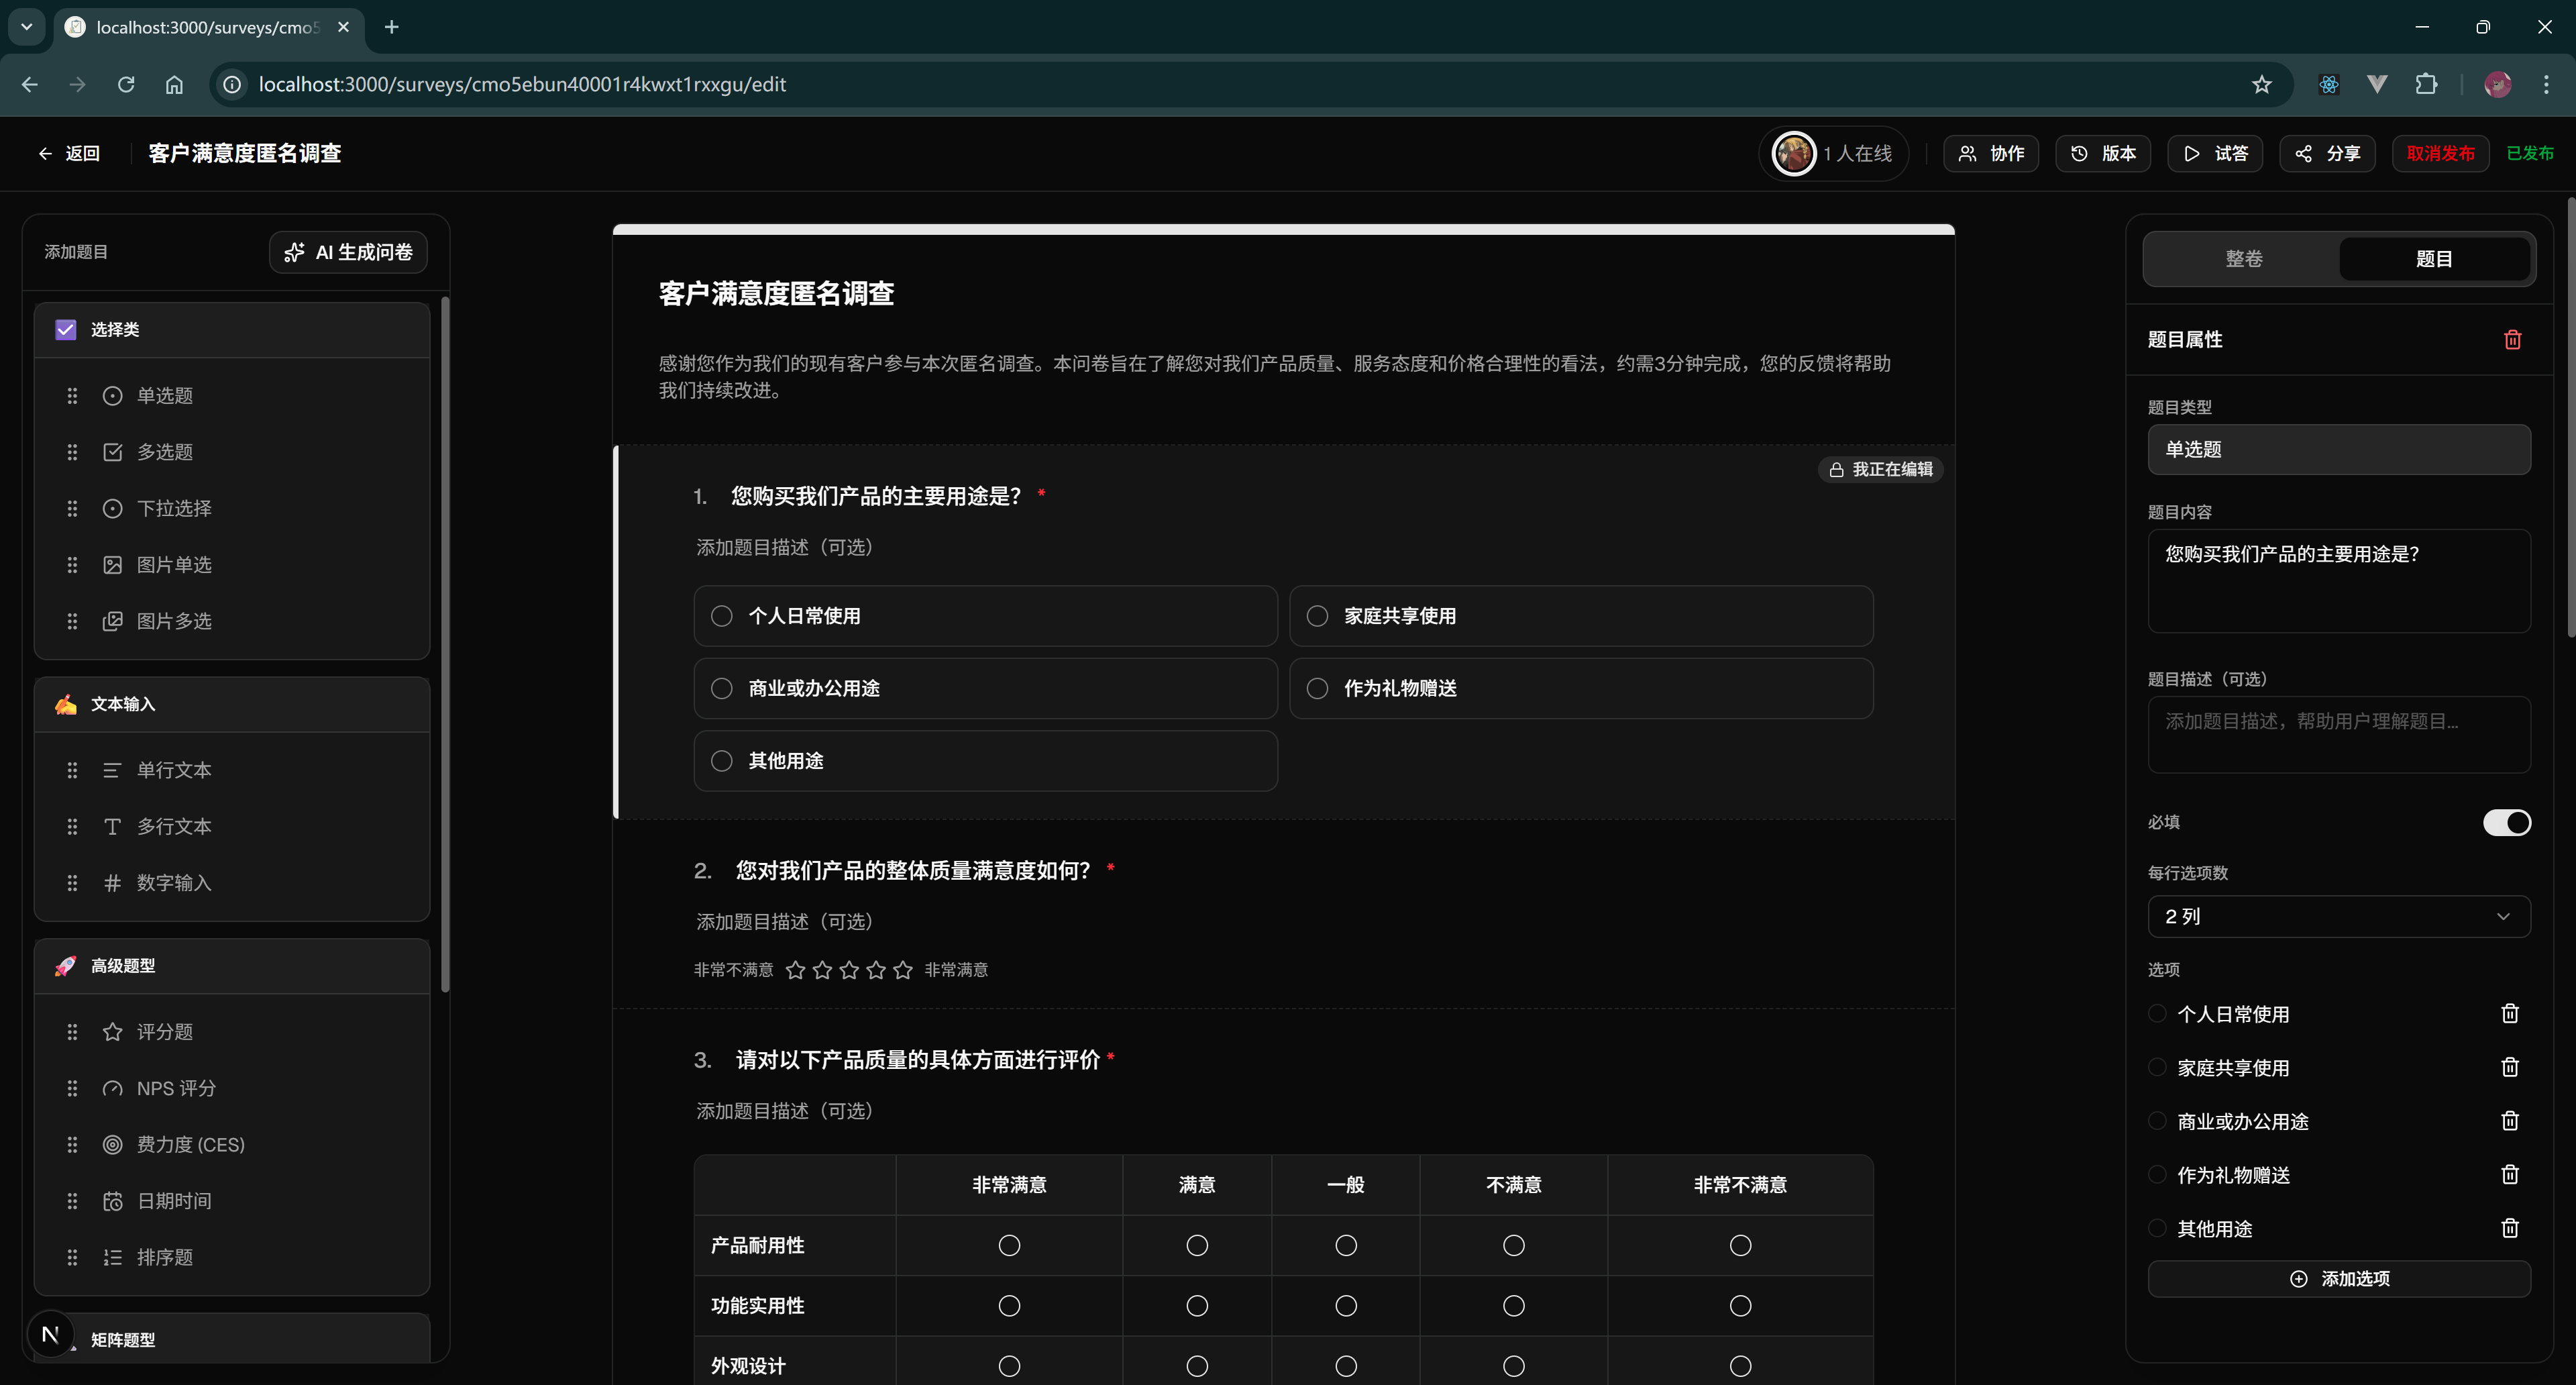
\includegraphics[width=0.95\textwidth]{figures/screenshot-editor.png}
\caption{问卷编辑器}
\end{figure}

\begin{figure}[H]
\centering
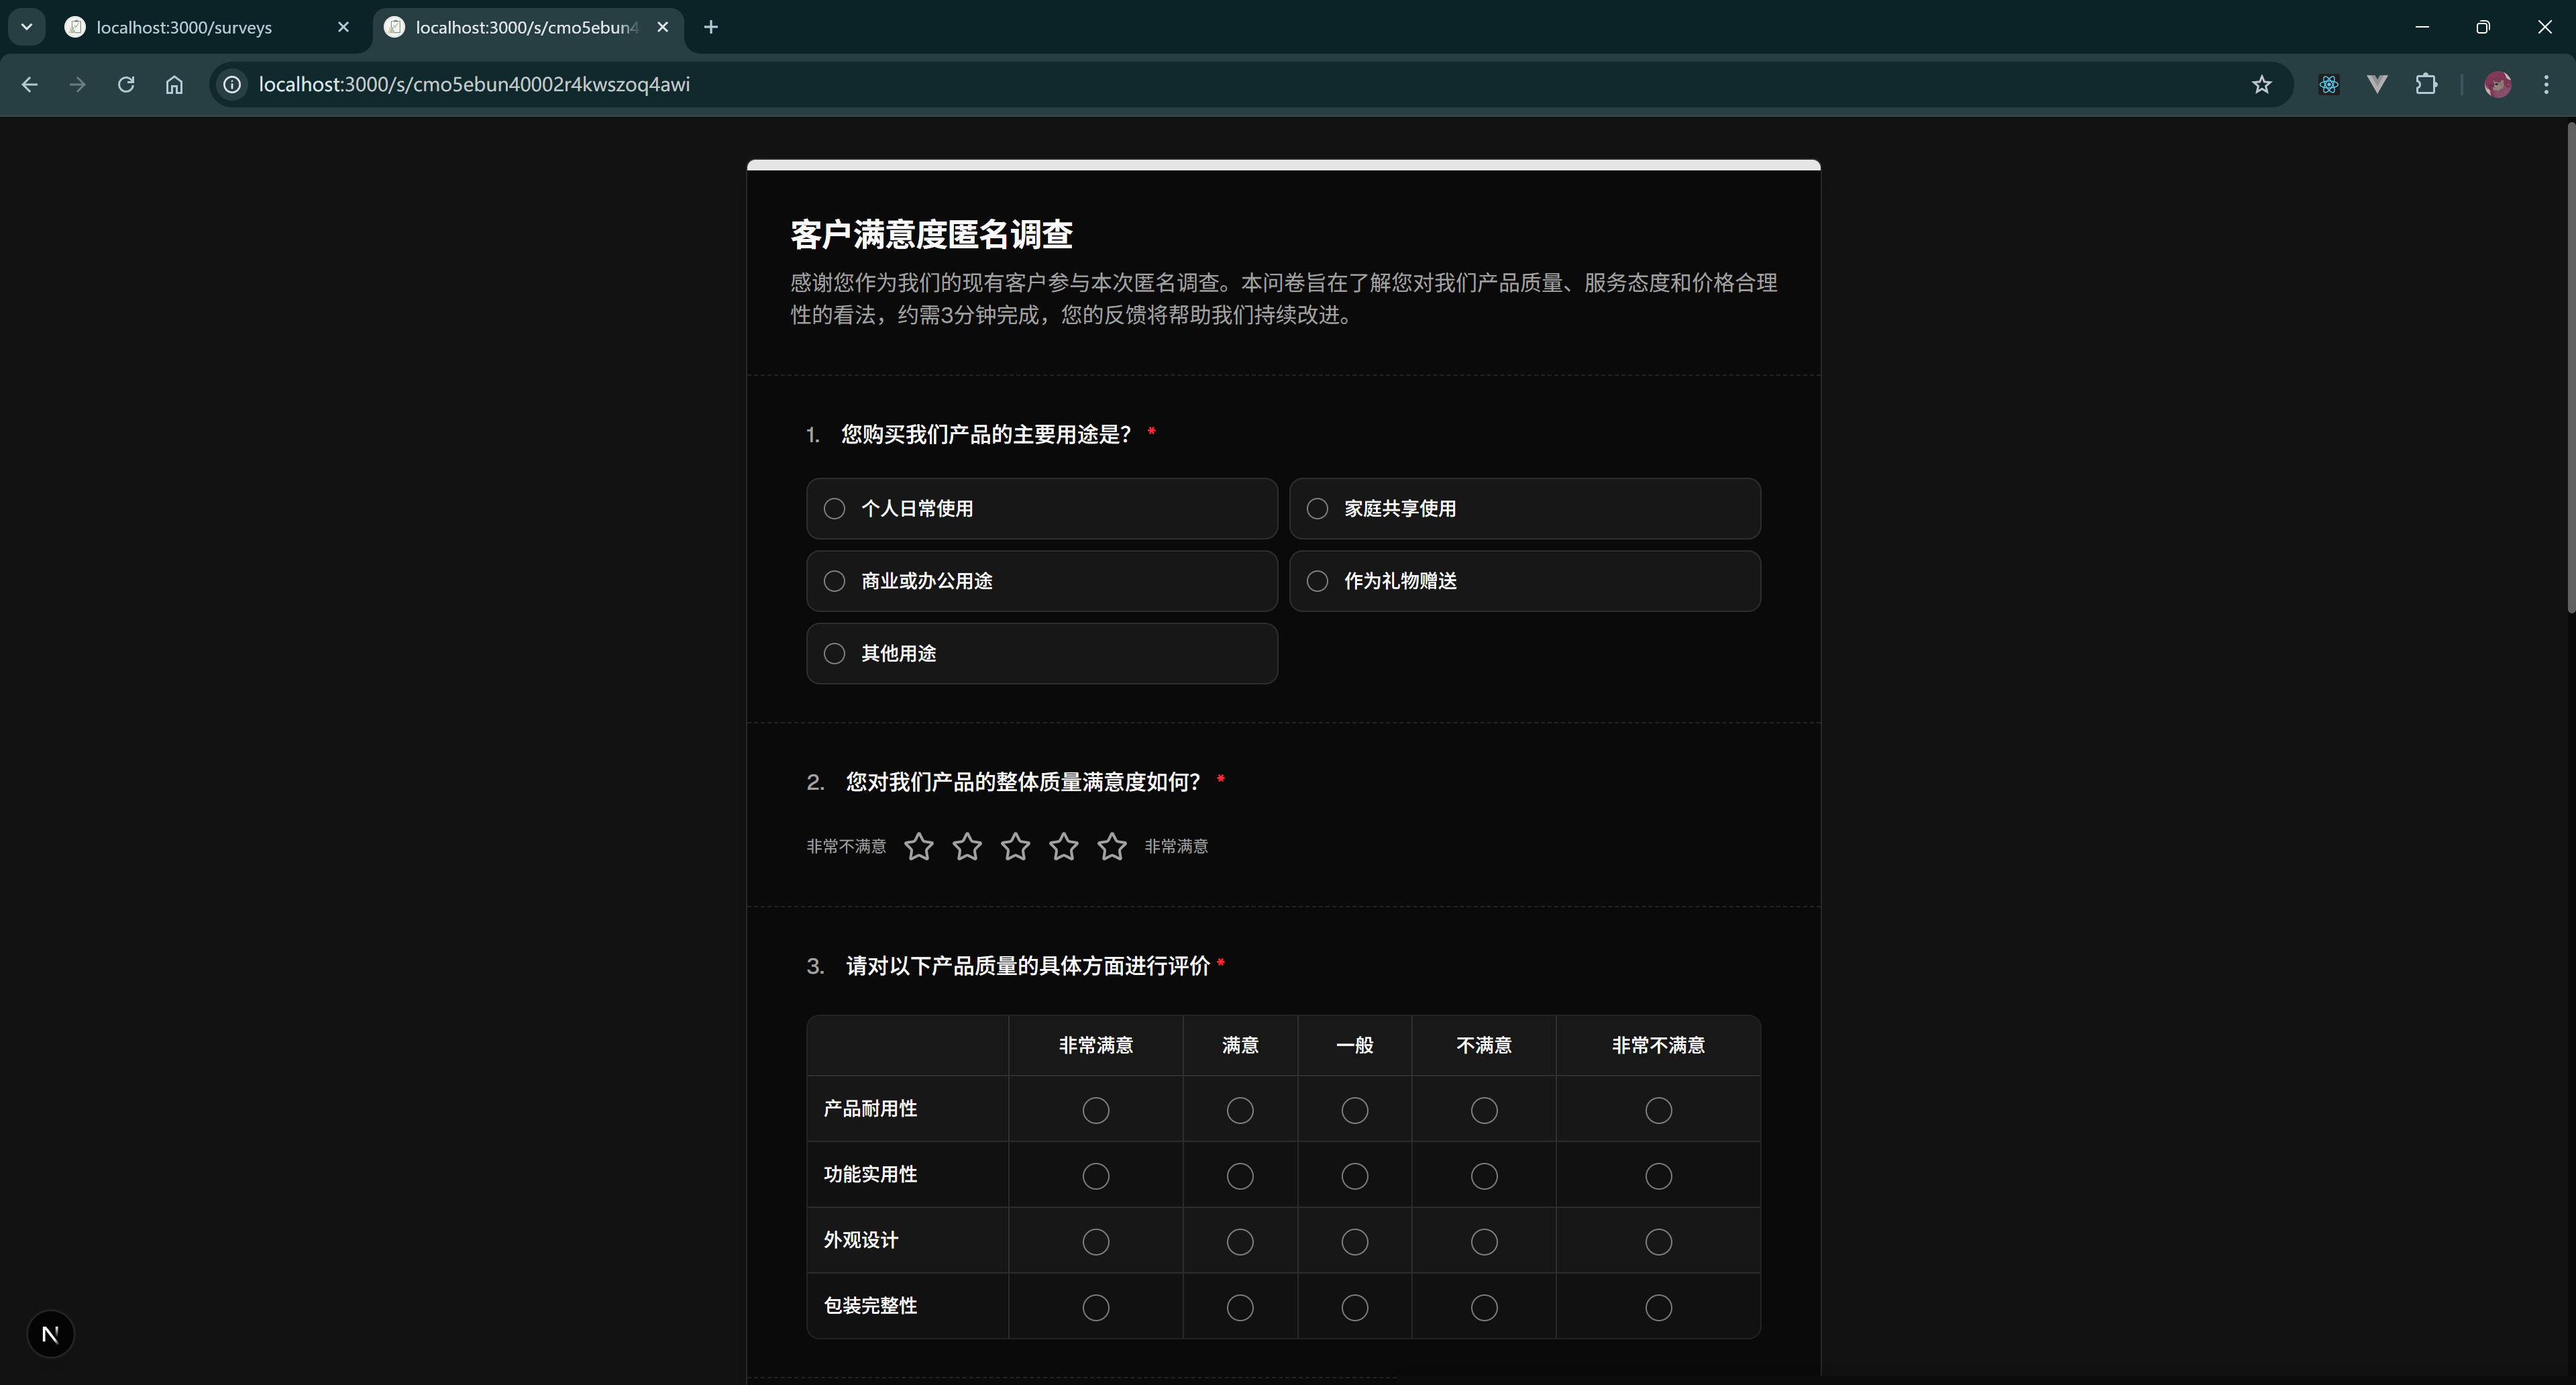
\includegraphics[width=0.95\textwidth]{figures/screenshot-public-form.png}
\caption{公开问卷填写页面}
\end{figure}

\begin{figure}[H]
\centering
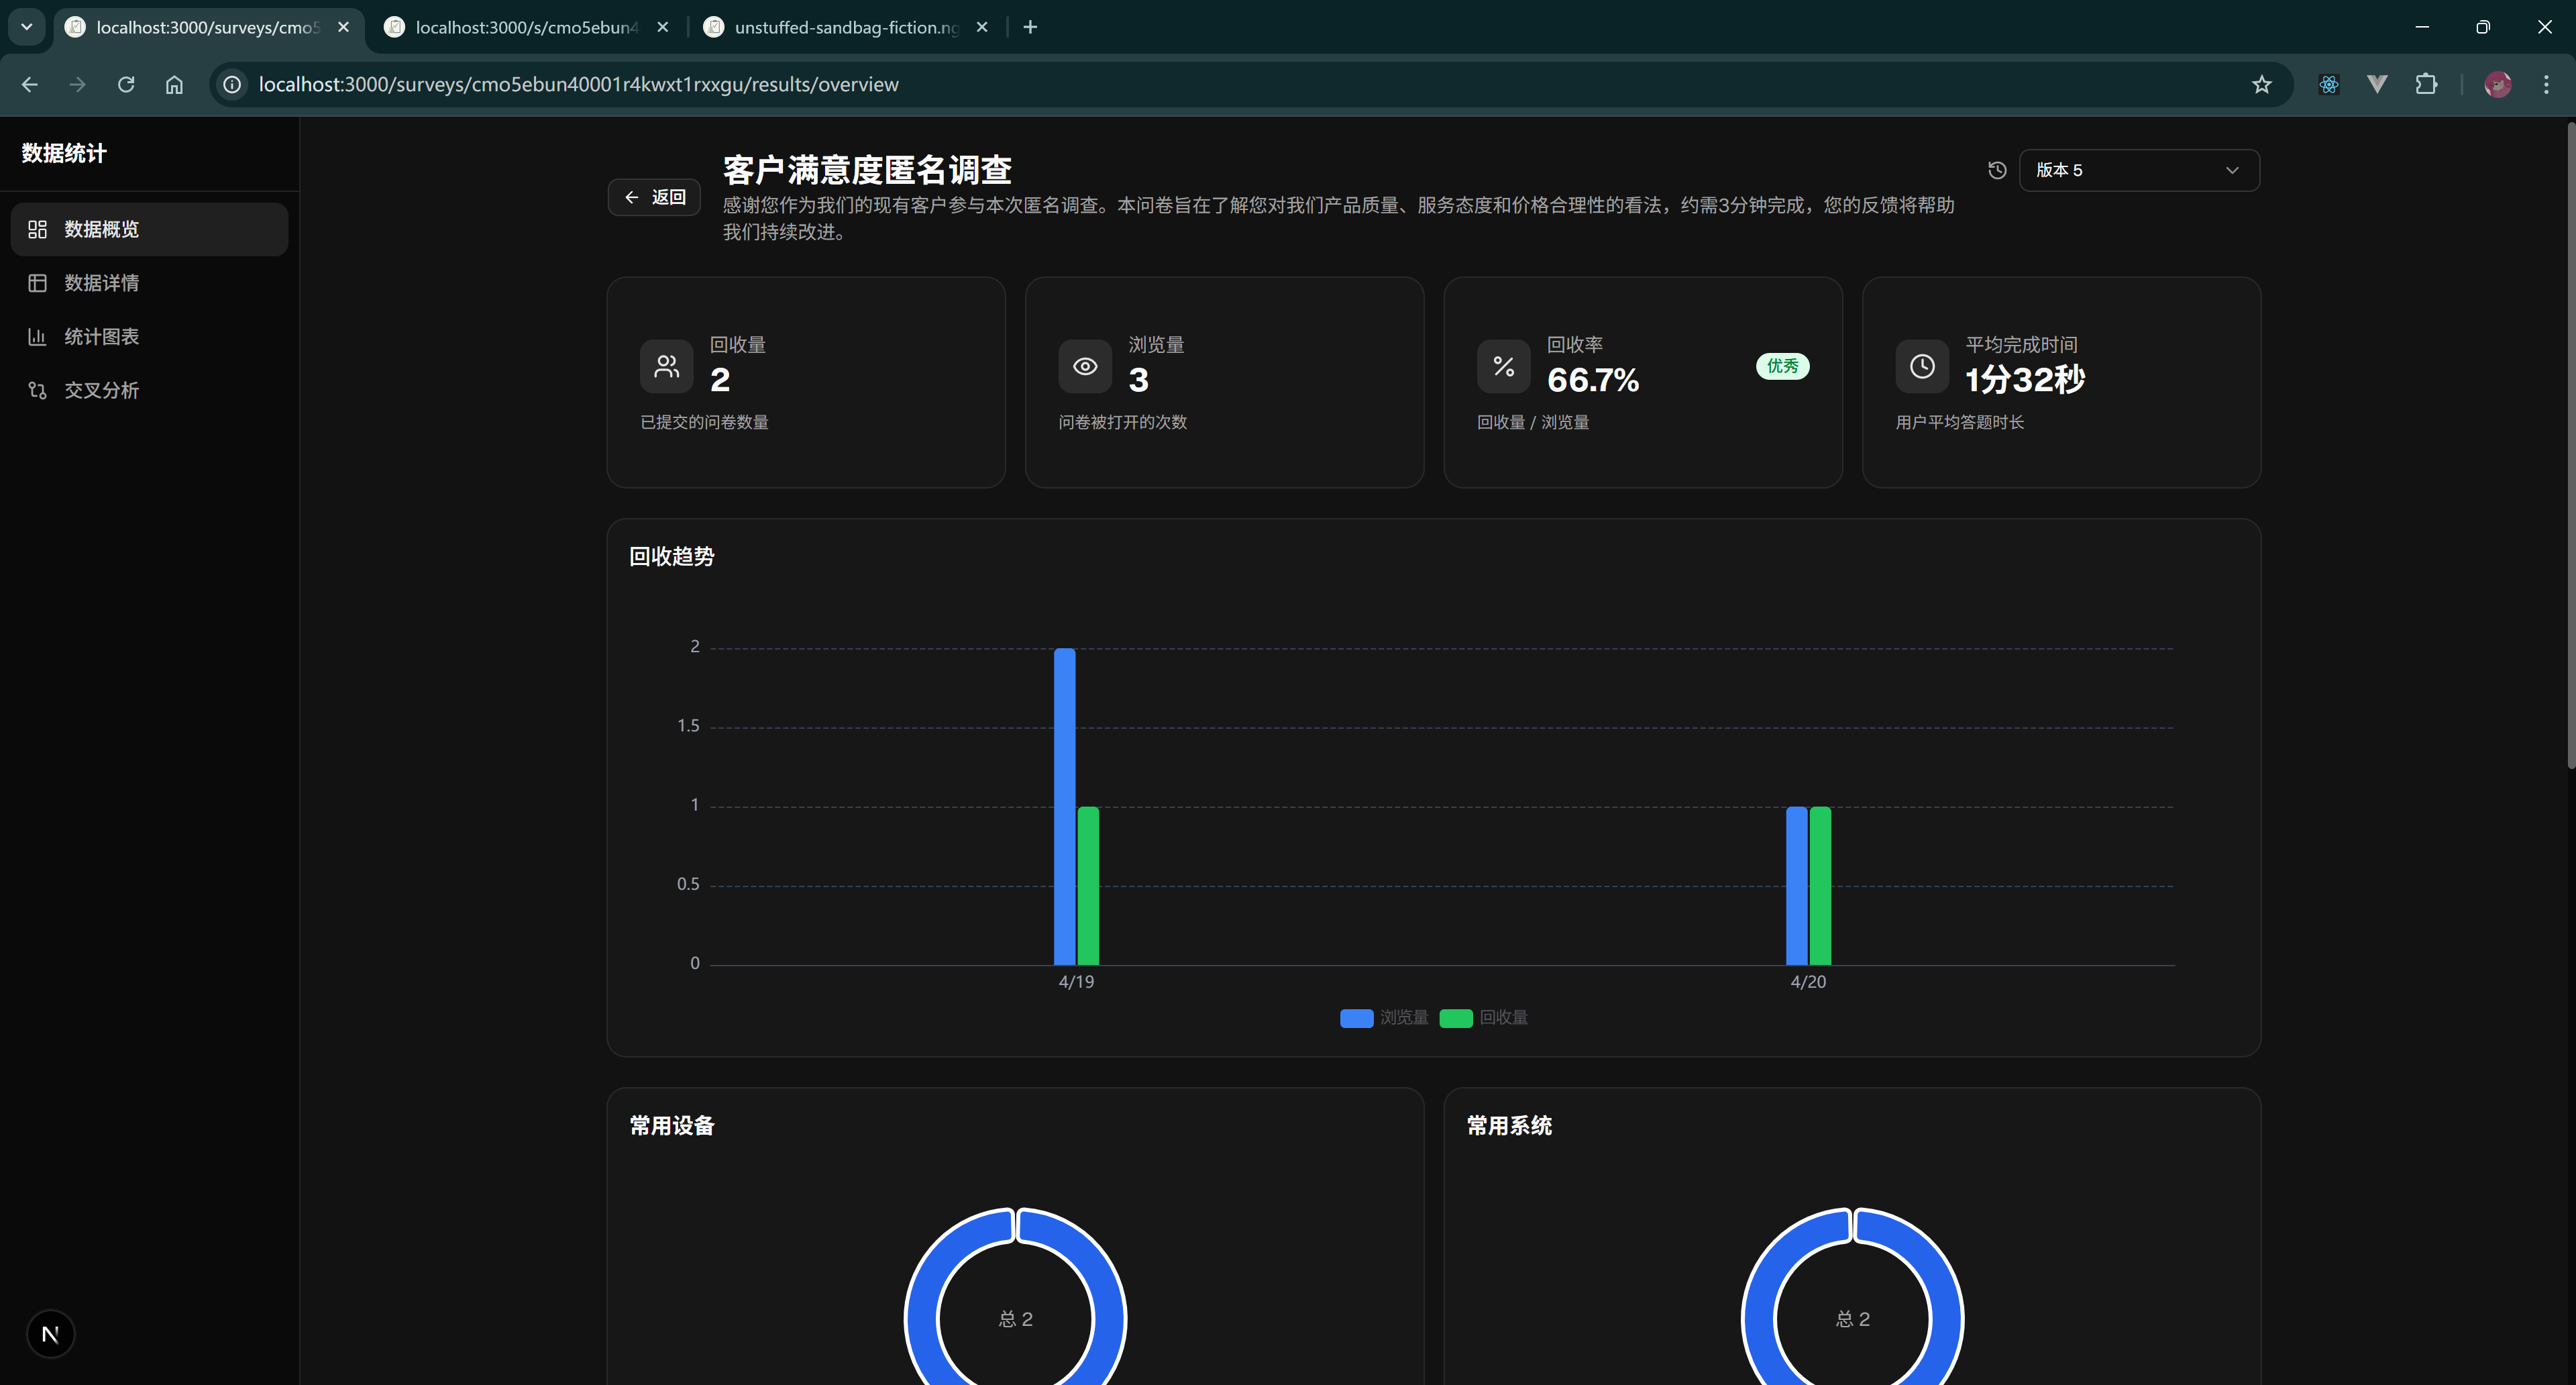
\includegraphics[width=0.95\textwidth]{figures/screenshot-results.png}
\caption{结果统计页面}
\end{figure}

\section{附录 C：项目结构}

\begin{minted}[linenos]{bash}
survey-test/
├── app/                    # Next.js App Router
│   ├── (auth)/            # 认证路由组
│   ├── (dashboard)/       # 仪表盘路由组
│   ├── (editor)/          # 编辑器路由组
│   ├── api/               # API 路由
│   ├── s/[token]/         # 公开问卷页面
│   └── invite/            # 邀请页面
├── components/            # React 组件
│   ├── auth/              # 认证组件
│   ├── editor/            # 编辑器组件
│   ├── questions/         # 题型组件
│   ├── ai/                # AI 组件
│   └── collaboration/     # 协作组件
├── lib/                   # 工具库
│   ├── auth.ts            # 认证配置
│   ├── editor-store.ts    # 编辑器状态
│   ├── questions/         # 题型系统
│   └── ai/                # AI 相关
├── hooks/                 # 自定义 Hooks
├── prisma/                # Prisma 配置
│   └── schema/            # 数据模型
├── docs/                  # 项目文档
├── thesis/                # 毕业论文
└── package.json           # 项目配置
\end{minted}
\captionof{listing}{项目目录结构}


\end{document}
